\chapter{Estimación de los fondos} \label{cap:fondos}


A partir de las muestras MC, como se describe en {\XXX}, se estima que la
contribución dominante de fondos del Modelo Estándar sea la producción de
{\wgam} y {\ttgam}. En la {\SRL} también se espera una contribución de procesos
de {\ttbar} en los que un electrón es mal identificado como fotón.

La estrategia general para la estimacion de los fondos del SM en este analisis
consistio en estimar los fondos provenientes de electrones o jets mal identificados como
fotones a partir los datos observados.

\hl{Aca decir que tales fondos DD, tales MCcorr y el resto MC}



%% , seguido de la producción de fotones con energía faltante instrumental.




\section{Fondos irreducibles}

Se definen tres regiones de control para determinar la normalización del MC de
{\wgam} ({\CRW}), {\ttgam} ({CRT}) y fotones ({CRQ}). Cada una de estas regiones
de control son dominadas por cada uno de estos fondos.

Los cortes de selección se mantienen lo mas similares posibles a la
correspondiente SR para minimizar el efecto de la extrapolación. Los fondos
debidos a la mal identificación de electrones y jets se estiman a partir de
métodos basados en los propios datos observados, descriptos en ...


\section{Fotones directos (+ jet)}

Definicion de la CRQ

\section{Electrones identificados como fotones} \label{sec:efakes}

En los casos en que un electrón de alto {\pt} sea mal identificado como un
fotón, estos eventos pueden entrar en alguna de las SR. Esta contaminación
proviene generalmente de procesos del SM como $W(\to e\nu)$+ jets, $Z(\to ee)$ +
jets y {\ttbar}.

Como la descripción del material del detector no es perfecta en las simulaciones Monte Carlo,
la estimación de este fondo se realiza a partir de los datos, como:
%% Para estimar este fondo se multiplica el número de eventos con un electrón observados
%% en la región CSE por la fracción de misidentificacion de fotón a electrón.

\begin{equation}
  N_{e\to\gam}^{\mathrm{SR}} = \feg \quad N_e^{\mathrm{SR}}
\end{equation}
%
donde $N_e^{\mathrm{SR}}$ es el número de eventos en la muestra de electrones
obtenida invirtiendo el rol de fotones y electrones en la selección de la región
de señal. Un electrón aislado de alto {\pt} es requerido, y fotones de señal son
vetados. Y {\feg} es la probabilidad de que electrón sea identificado
erróneamente como un fotón.

Para estimar la probabilidad de identificar erroneamente un electrón como un
fotón {\feg} se utiliza un método llamado \emph{tag and probe}, en una muestra
de eventos de datos {\Zee} que pasan el mismo trigger de fotones que utiliza el
análisis y la misma preselección (ver \cref{sec:event_baseline}). Adicionalmente, se
aplica un corte de $\met < 40 \gev$ para reducir la posible contaminación de
fotones reales de eventos de {\wgam}.

El método consiste en seleccionar un electrón (el electrón \emph{tag}). Este
electrón debe pasar un criterio de identificación \emph{tight} y que tener $20
\gev < \pt < 125 \gev$. Luego se busca un segundo candidato a electron o foton
(el objeto \emph{probe}). Este puede ser un electrón \emph{tight} o un fotón
\emph{tight}, ambos con $\pt > 125\gev$ y satisfaciendo los requerimientos de
aislamiento que se describen en la \cref{sec:obj_selection}\note{Chequear}.

Los valores de la masa de los pares de objetos seleccionados son guardados
separadamente para los tres casos posibles: dos electrones, un electrón y un
fotón convertido, o un electrón y fotón no-convertido. En los tres casos se
puede ver un pico alrededor del valor de la masa del bosón $Z$ ($m_Z \sim 91
\gev$).

Como el bosón $Z$ no puede decaer directamente en un electrón y un fotón, los
pares electrón-fotón que aparecen bajo el pico del $Z$ corresponden a electrones
mal identificados. Sin embargo, lo mismo aplica a otras partículas que decaen en
pares de electrones y por lo tanto es necesario utilizar algun metodo de
sustraccio del fondo. Este deberá también tener en cuenta la contaminación por
combinaciones aleatorias.

La probabilidad de identificacion erronea {\feg} puede estimarse entonces como:

\begin{equation}\label{eq:efakerate}
  \feg = \frac{N_{e\gam}}{N_{ee}}
\end{equation}
%
donde $N_{e\gam}$ ($N_{ee}$) es el número de pares electrón-fotón
(electrón-electrón) encontrados bajo el pico del bosón $Z$ en la distribución de
la masa invariante, definida en el rango $81 < m_{ex} < 101 \gev$. Para obtener
el número de eventos $N_{ex}$, se realiza un ajuste de la distribución de la
masa invariante para los dos tipos de eventos utilizando un modelo de
señal+fondo. Este procedimiento se lleva a cabo de forma separada para fotones
convertidos y no-convertidos, y en clases del {\abseta} de los objetos
\emph{probe}. El bajo numero de eventos disponibles hace imposible utilizar
clases de {\pt}, aunque de esta forma la estimación es conservativa ya que la
probabilidad de identificacion erronea decrece con el {\pt} del electrón
\cite{Kuhl:1604846}.

Como modelo de señal se utiliza la suma de función \emph{Crystall-Ball} y una
Gausiana, mientras que para el modelo de fondo se utiliza un polinomio de grado
dos. En la \cref{fig:invmass_pairs} se puede ver las distribuciones de la masa
invariante para pares de $ee$ y $e\gam$, para la selección inclusiva.

\begin{figure}[!htbp]
  \centering

  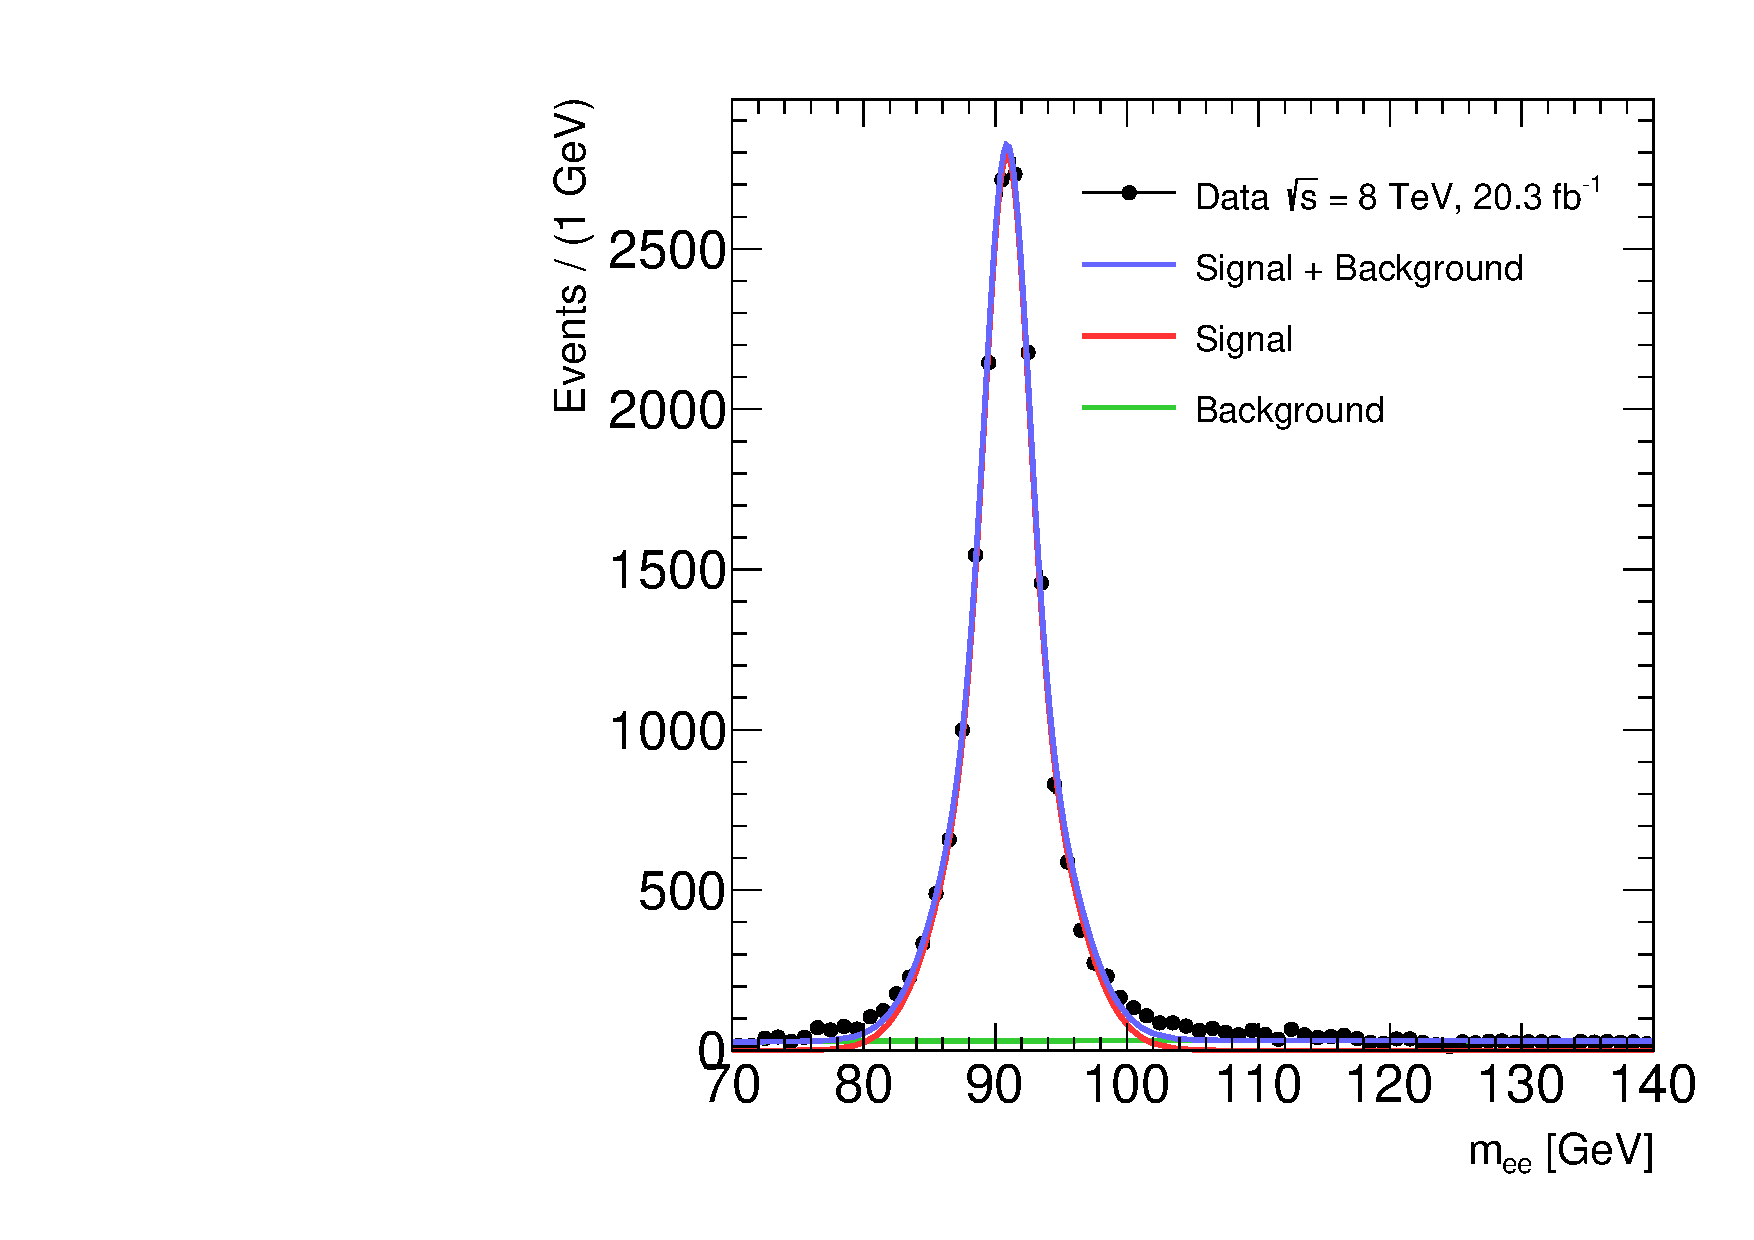
\includegraphics[width=0.49\textwidth]{figures/Fit_mee_efakes_Data_all}
  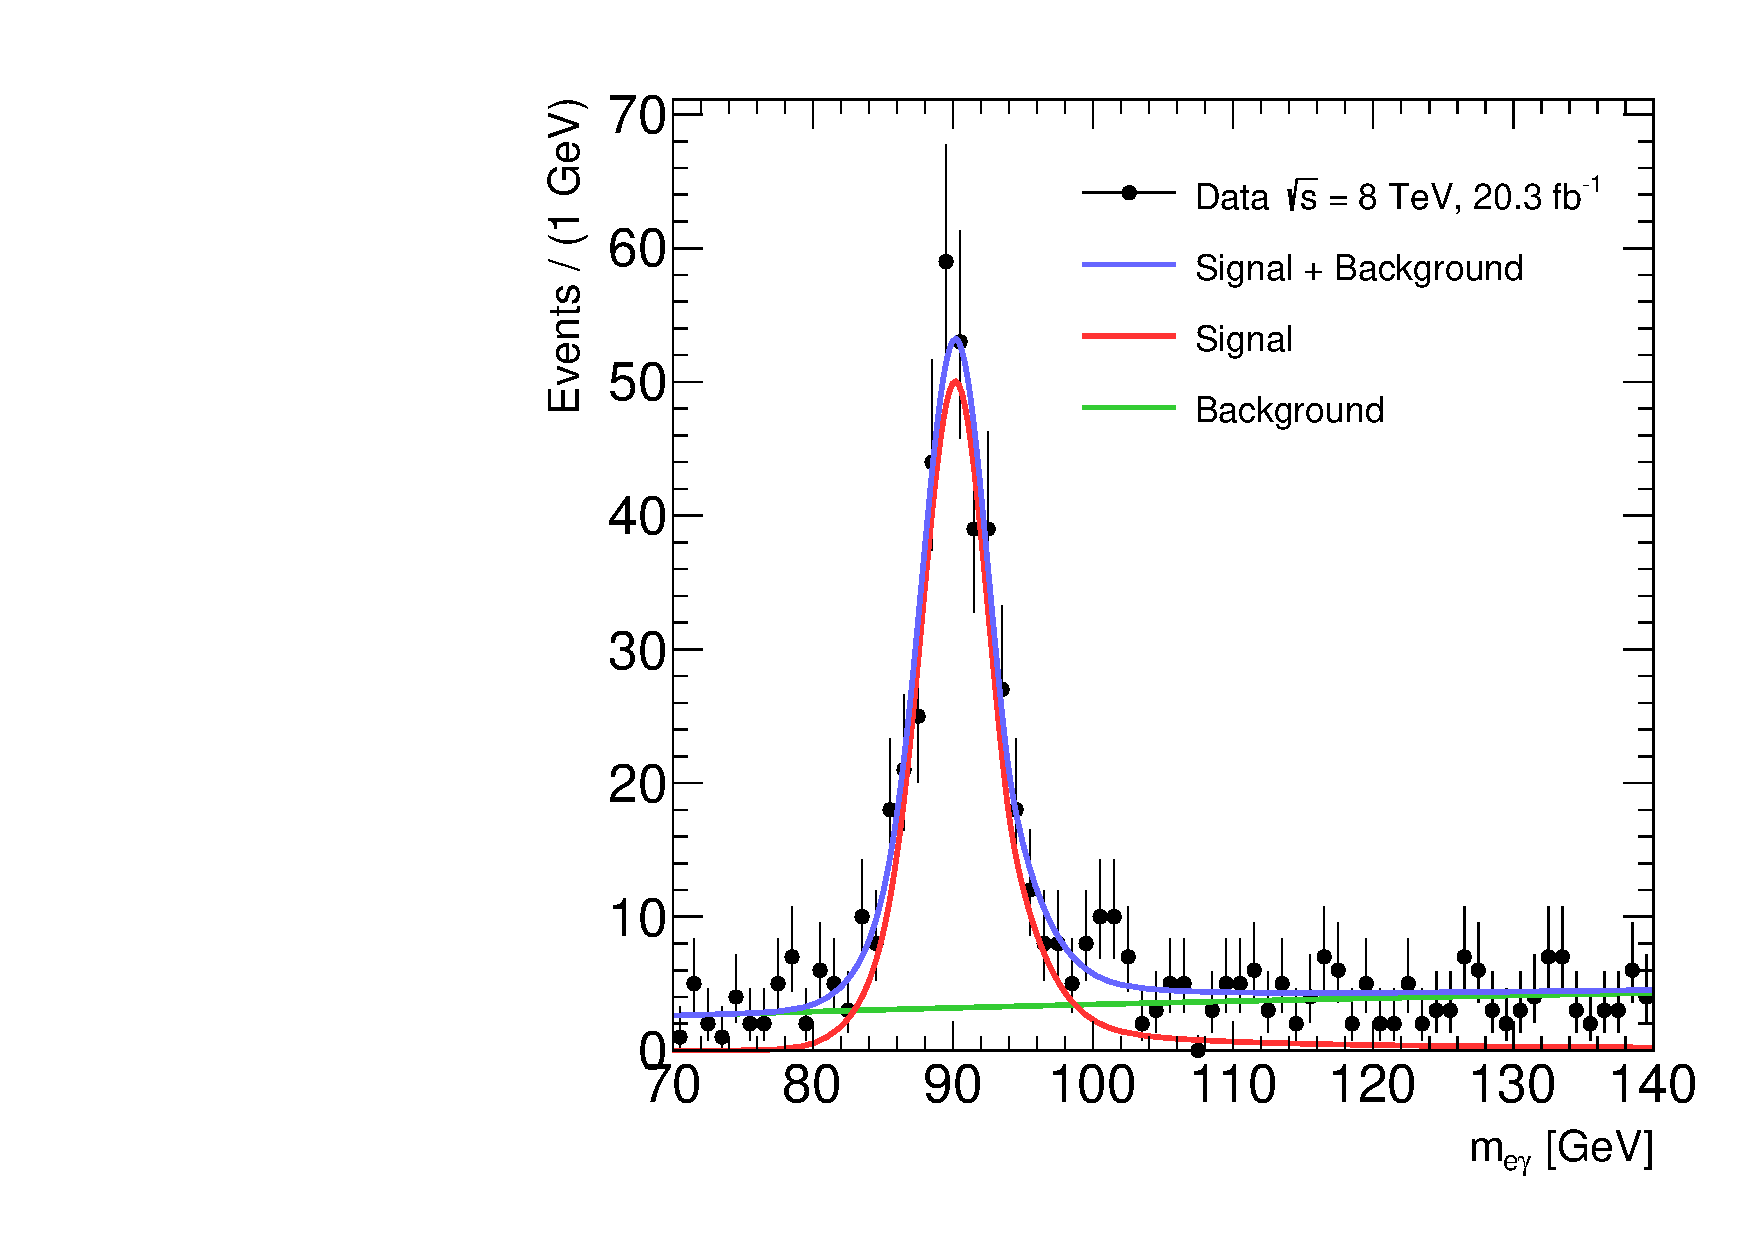
\includegraphics[width=0.49\textwidth]{figures/Fit_meg_efakes_Data_all}
  \caption{Distribuciones de la masa invariante de los pares de
    electrón-electrón (izquierda) y electrón-fotón (derecha). Se puede ver también el ajuste
    con el modelo de señal + fondo.}
  \label{fig:invmass_pairs}

\end{figure}

La probabilidad de identificación errónea se muestra en la \cref{fig:efake_eta},
como función del {\abseta} del objeto \emph{probe} para ``fotones'' convertidos
y no-convertidos. Este factor crece con {\abseta}, lo cual esta correlacionada
con el incremento en el material del detector atravesado por los electrones y el
incremento en la tasa de reconstrucción de fotones convertidos con una sola
traza.

El {\feg} calculado a partir de los datos es comparado con el calculado a partir
de muestras MC de eventos de {\Zee} producidas con los generadores {\sherpa} y
{\powheg}. Se encuentra un buen acuerdo para todos los casos dentro de sus incertezas.
Los valores calculados de {\feg} pueden verse en la \cref{tab:efake_eta}, y \cref{tab:efake_uc} para fotones
convertidos y no-convertidos de forma separada.

\begin{figure}[!htbp]
  \centering

  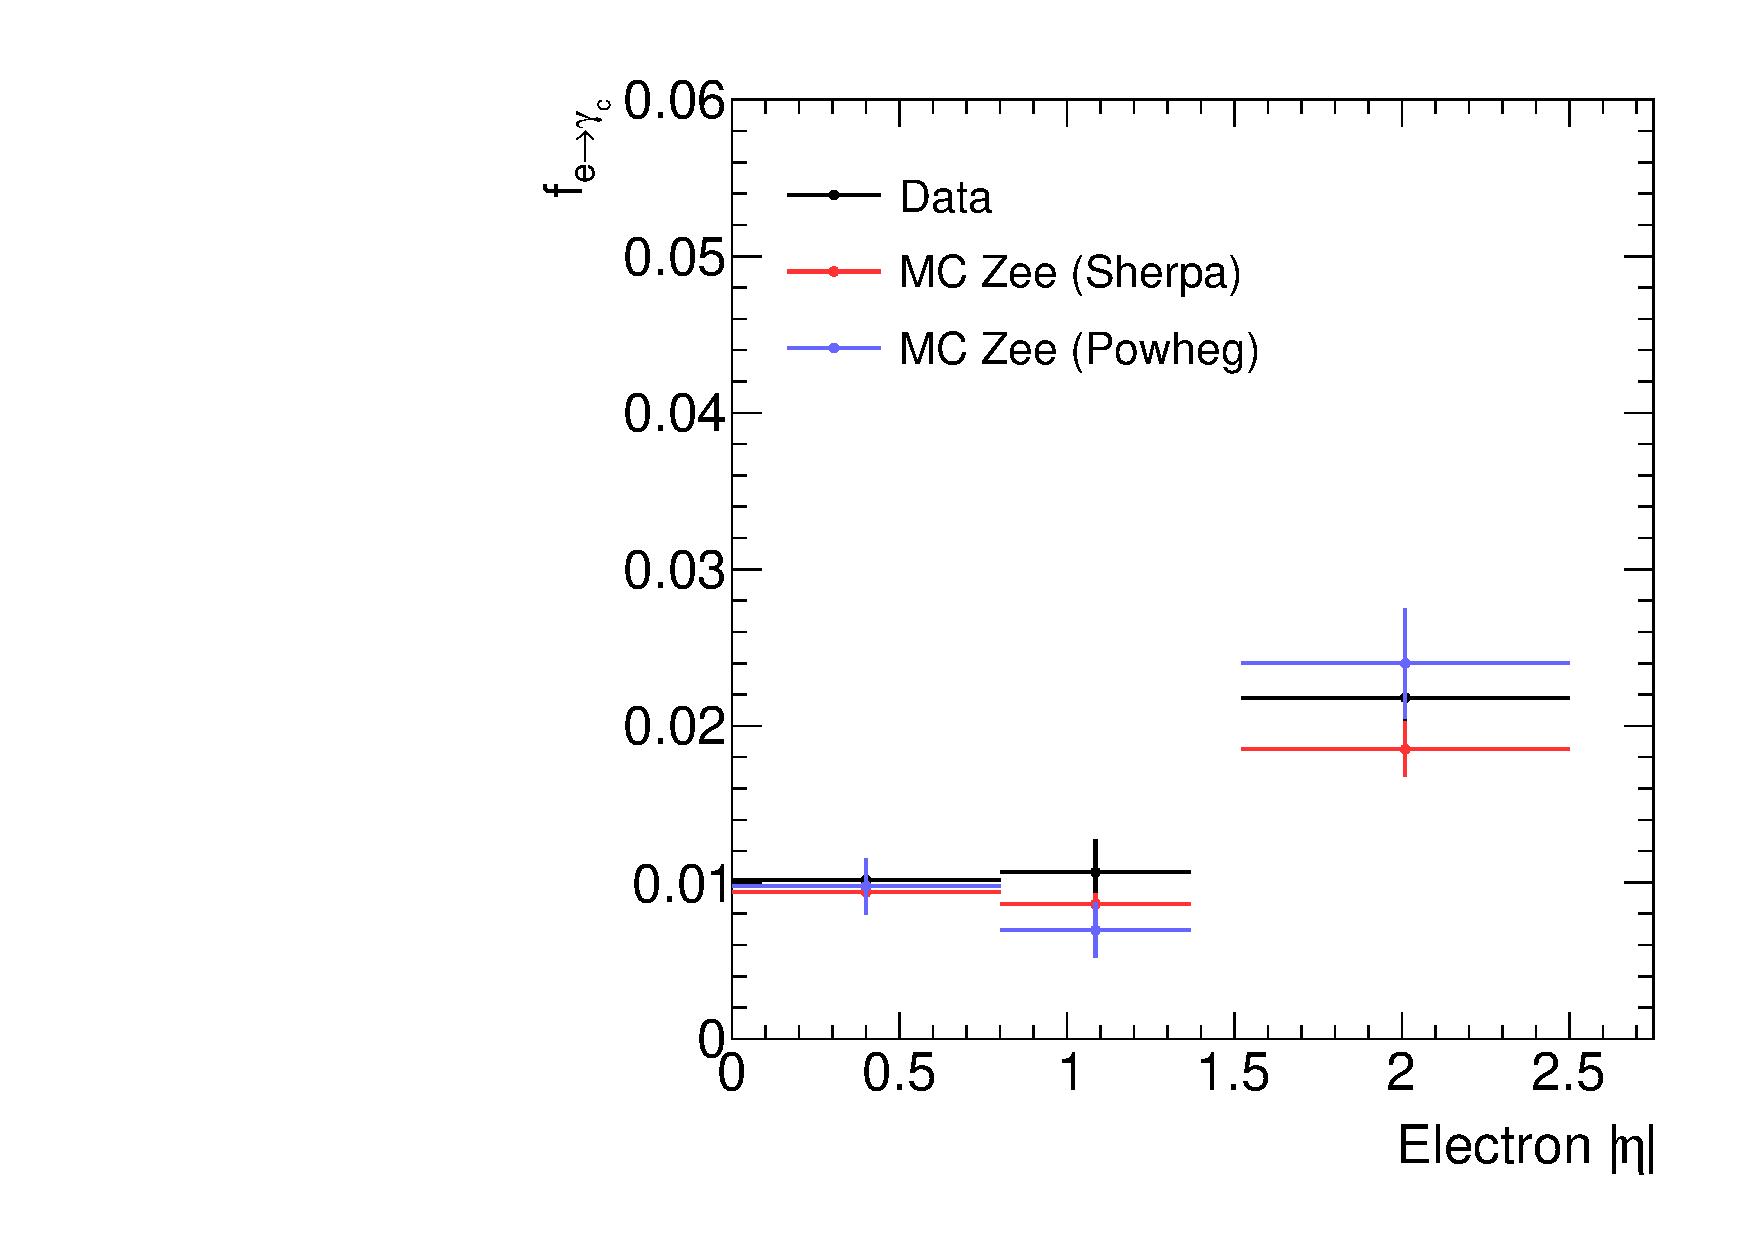
\includegraphics[width=0.45\textwidth]{figures/fegc_feta}
  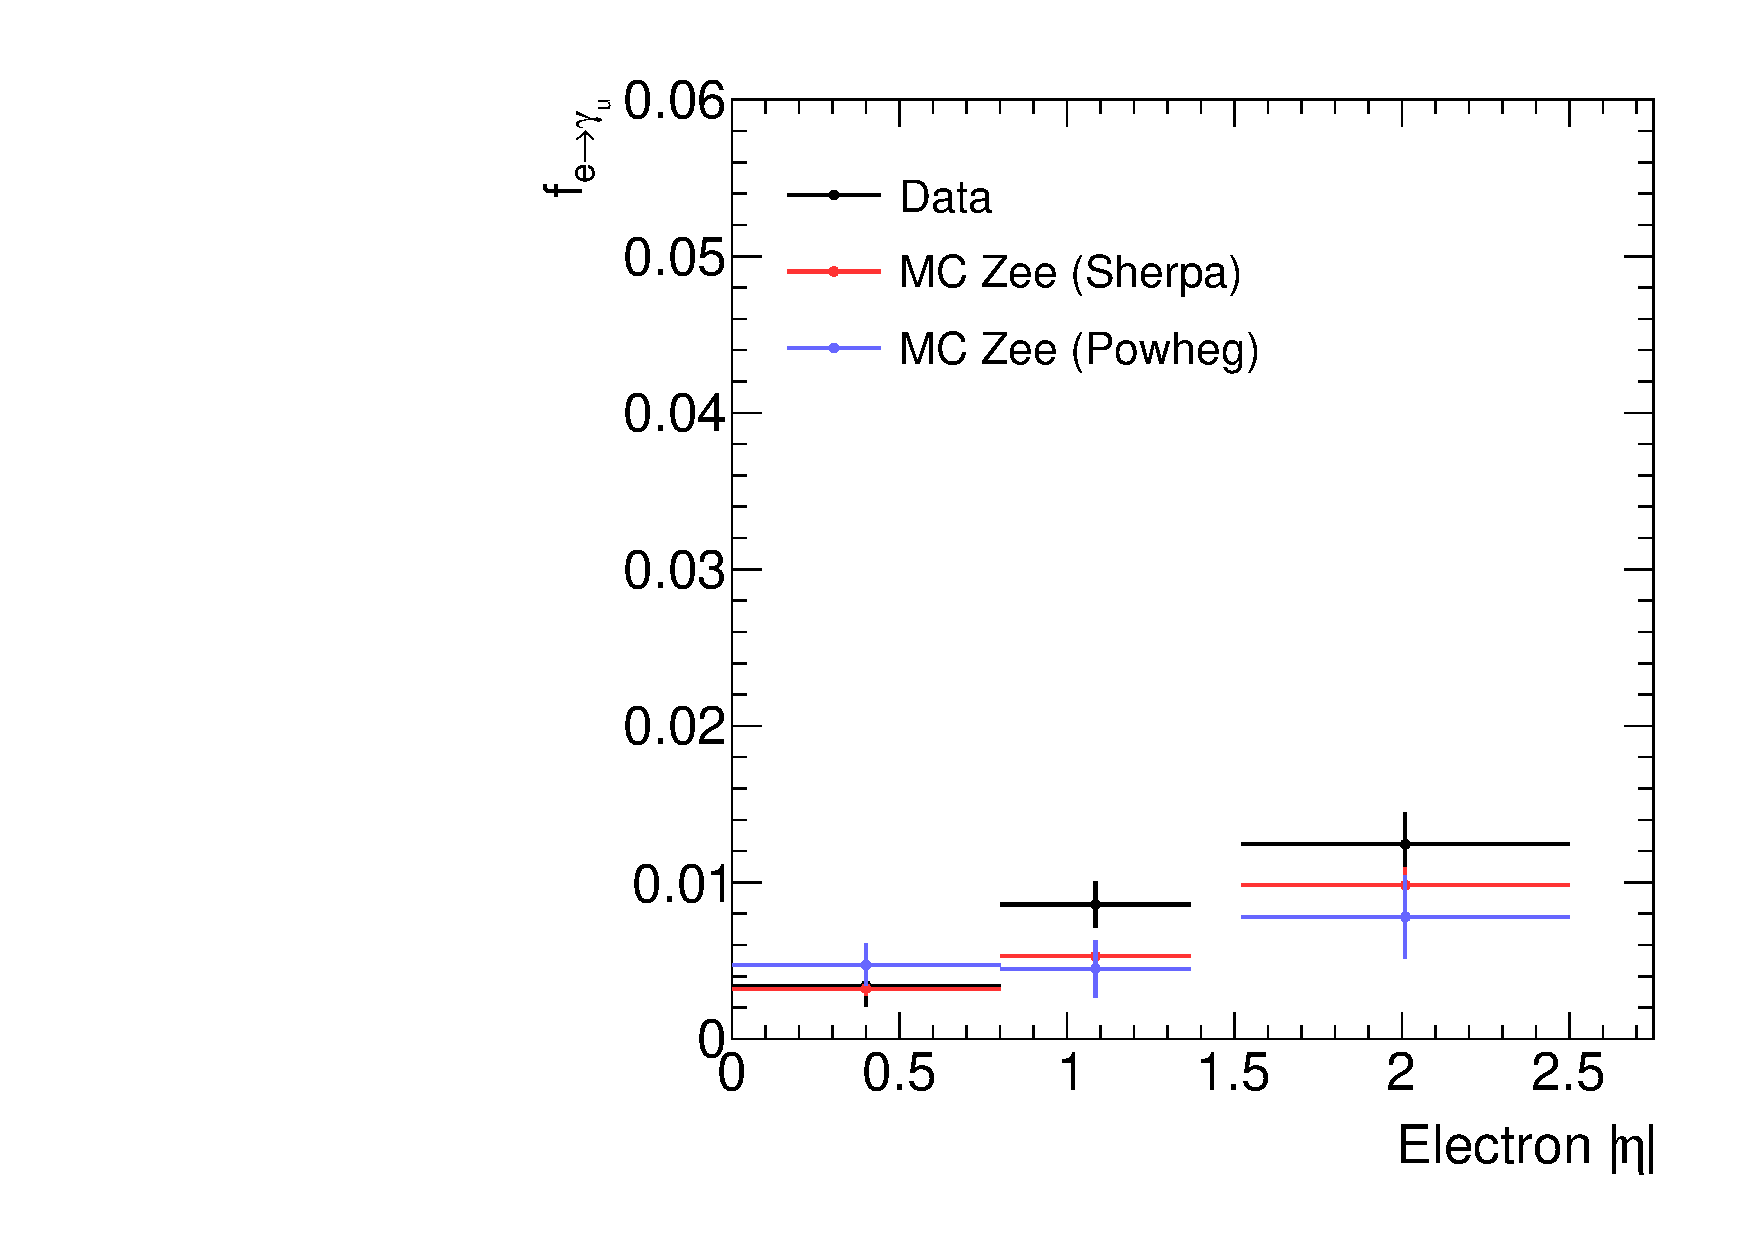
\includegraphics[width=0.45\textwidth]{figures/fegu_feta}

  \caption{Probabilidad de que un electrón real sea identificado como un fotón convertido (izquierda)
    y un fotón no-convertido (derecha), como función de la pseudo-rapidez del objeto \emph{probe}. El valor
    calculado a partir de los datos es comparado con el valor calculado con las muestras MC de eventos de {\Zee} utilizando
    dos generadores distintos.}
  \label{fig:efake_eta}
\end{figure}


\begin{table}[!htbp]
  \centering
  \caption{Probabilidad de que un electrón real sea identificado como un fotón,
    como función de la pseudo-rapidez del objeto \emph{probe}. El valor
    calculado a partir de los datos es comparado con el valor calculado con las
    muestras MC de eventos de {\Zee} utilizando dos generadores distintos.}
  \label{tab:efake_eta}

  \begin{tabular}{x{0.16\textwidth}x{0.21\textwidth}x{0.21\textwidth}x{0.21\textwidth}}
    \hline
                          & Datos             &  {\Zee} (\sherpa) & {\Zee} (\powheg) \\
    \hline
    $0 < |\eta| < 0.8$    & $0.014 \pm 0.002$ & $0.012 \pm 0.001$ & $0.014 \pm 0.002$ \\
    $0.8 < |\eta| < 1.52$ & $0.018 \pm 0.003$ & $0.014 \pm 0.001$ & $0.011 \pm 0.003$ \\
    $1.52 < |\eta| < 2.5$ & $0.033 \pm 0.006$ & $0.027 \pm 0.002$ & $0.032 \pm 0.006$ \\
    Inclusivo             & $0.019 \pm 0.001$ & $0.016 \pm 0.001$ & $0.017 \pm 0.002$ \\
    \hline
  \end{tabular}

\end{table}

\begin{table}[!htbp]
  \centering
  \caption{Probabilidad de que un electrón real sea reconstruido como un fotón
    convertido o no-convertido. El valor calculado a partir de los datos es
    comparado con el valor calculado con las muestras MC de eventos de {\Zee},
    utilizando dos generadores distintos.}
  \label{tab:efake_uc}

  \begin{tabular}{x{0.16\textwidth}x{0.21\textwidth}x{0.21\textwidth}x{0.21\textwidth}}
    \hline
                       & Datos              & {\Zee} (\sherpa)        & {\Zee} (\powheg)        \\
    \hline
    $f(e\to \gamma_u)$ & $0.007 \pm 0.001$ & $0.005 \pm 0.001$ & $0.005 \pm 0.001$ \\
    $f(e\to \gamma_c)$ & $0.013 \pm 0.001$ & $0.011 \pm 0.001$ & $0.011 \pm 0.002$ \\
    $f(e\to \gamma)$   & $0.019 \pm 0.001$ & $0.016 \pm 0.001$ & $0.017 \pm 0.002$ \\
    \hline
  \end{tabular}

\end{table}

Para estimar la incerteza sistemática del método utilizado, el factor {\feg} fue
calculado variando el tamaño de la ventana de masa del $Z$, y sin la sustracción
del fondo. Como se aprecia en la \cref{tab:efake_syst}, en el caso de no
realizar la sustracción del fondo, es donde se obtiene la mayor variación y por
lo tanto se utiliza ese valor como la incerteza sistemática del método, a pesar
de que resulta conservativo.

\begin{table}[!htbp]
  \centering
  \caption{Probabilidad de que un electrón real sea reconstruido como un fotón
    convertido o no-convertido, para variaciones del método original.}
  \label{tab:efake_syst}

    \begin{tabular}{x{0.14\textwidth}x{0.22\textwidth}x{0.22\textwidth}x{0.22\textwidth}}
    \hline
            &  $71 < m_{ee} < 111 \GeV$ & $86 < m_{ee} < 96$ & Sin sustraccion del fondo  \\
    \hline
    $f(e\to \gamma_u)$ & $0.007 \pm 0.001$ & $0.007 \pm 0.001$ & $0.012 \pm 0.001$ \\
    $f(e\to \gamma_c)$ & $0.013 \pm 0.001$ & $0.012 \pm 0.001$ & $0.012 \pm 0.001$ \\
    $f(e\to \gamma)$   & $0.019 \pm 0.001$ & $0.019 \pm 0.001$ & $0.024 \pm 0.001$ \\
    \hline
  \end{tabular}

\end{table}


El valor calculado del factor de identificación errónea de electrón en fotón
({\feg}) resulta entonces el que se muestra en la \cref{tab:efake_final}.

\begin{table}[!htbp]
  \centering
  \caption{Valor calculado final para el factor {\feg}, como función de $\eta$.}

  \begin{tabular}{x{0.2\textwidth}x{0.6\textwidth}}

    \hline
     Región                &  $f(e\to \gamma)$  \\
    \hline
      $0 < |\eta| < 0.8$     & $ \quad  0.014 \pm 0.002 \stat\ \pm 0.005 \syst\ $ \\
      $0.8 < |\eta| < 1.52$  & $ \quad  0.018 \pm 0.003 \stat\ \pm 0.004 \syst\ $ \\
      $1.52 < |\eta| < 2.5$  & $ \quad  0.033 \pm 0.006 \stat\ \pm 0.008 \syst\ $ \\
    \hline
  \end{tabular}
  \label{tab:efake_final}
\end{table}

%% FINAL ESTIMATION IN SIGNAL REGIONS
%% \subsubsection{Estimación final en las regiones de señal} \label{sec:efakes_estimation}

%% En la region CSE$_L$, there are 28 events observed, which then correspond to an estimation for this background of $N^\text{SR2}_\text{efakes} = 0.38\, \pm\, 0.07$.
%% In CSE3, given the harder \MET\ cut, there is no observed event in the electron sample for the data analised.

%number of electron events observed by the fake factor computed in data in three $\eta$ regions, [0, 0.8], [0.8, 1.52], [1.52, 2.5].

%% In SR2, only one electron event is observed, which then correspond to an estimation for this background of $N^\text{SR2}_\text{efakes} = 0.02\, \pm\, 0.02$.
%% In SR3, given the harder \MET\ cut, there is no observed event in the electron sample for the data analised.
%% The MC predicts this background to be indeed rather small (actually no event survived the SR3 selection with
%% the available statistics), which is consistent with the observed limit of $<0.02$ events. The estimation of
%% electron fake background for SR3 is then $N^\text{SR3}_\text{efakes} = 0.0^{+0.03}_{-0.0}$, which accomodates the total fake rate uncertainty.

%As a conservative estimate, the last observed yield in the \MET distribution (one event at 200\gev) is taken. This way, it translates to the same estimation as for SR2, after the \etogam\ fake factor is applied.


%The total number of electron events, summed over all $\eta$ bins is reported in \Tab \ref{tab:efake_yields}.
%From these, the number of \etogam\ events expected in the signal region is %$3.679\pm xx$,
%$0.828\pm yy$ and $0.679\pm zz$ events for SR2 and SR3 signal regions, respectively. Only statistical uncertainties are here considered. \tosolve{uncertainties!}%%The associated systematics are discussed in sec \ref{sec:syst_efakes}.
%
%\begin{table}[h!]
%  \centering
%    \caption{Number of misidentified electron events expected in the different signal regions. The unscaled number is weighted by
%    the electron-photon fake rate to get the final background yield from electron fakes in the three
%  analysis regions.}
%  \begin{tabular}{c|cc}
%    \hline
%    \hline
%    Signal region & Unscaled & Weighted  \\
%    \hline
%%    SR1 & $231$ & $3.679$ \\ %% \pm 0.251$ \\
%    SR2 & $57$ & $0.828$ \\ %% \pm 0.110$ \\
%    SR3 & $47$ & $0.679$ \\ %% \pm 0.100$ \\
%    \hline
%    \hline
%  \end{tabular}
%  \label{tab:efake_yields}
%\end{table}




%-----------
% Jet fakes
%-----------
\section{Jets identificados como fotones} \label{sec:jetfakes}

Los jets pueden ser mal identificados como fotones si fluctúan a uno o dos
{\pizero} con alto \pt, resultando en un objeto electromagnético indistinguible
de un solo fotón muy energético. Este fondo proviene mayoritariamente de
multijets, {\wjets} y eventos {\ttbar} decayendo semi leptónicamente, y puede
ser una fuente importante de contaminación. Como se espera que la tasa de mala
identificacion no este bien modelada por el MC, se la determina utilizando un
método a partir de los datos. La idea es utilizar las diferencias en la
distribución de energía de aislamiento esperada para fotones reales y falsos,
como se describe a continuación.

Para reducir significativamente este fondo proveniente de jets, para seleccionar
los fotones se utiliza un criterio de selección \emph{tight}, como se describe en
\cref{sec:pho_obj}. Esta selección incluye a todos los fotones reales y tienen
una moderada contaminación de jets. Es por definición un criterio mas ajustado
que el trigger de fotones utilizado para la toma de los datos, por lo que hay
una suficiente cantidad de candidatos a fotones de jets que van a fallar la
selección \emph{tight} pero van a satisfacer una selección intermedia. Estos
jets mas similares a un fotón real, llamados \emph{pseudo-fotones}, son útiles
para modelar los jets que pasan la selección total y la tasa de esta
contaminación.

%Pseudo-photons are here defined as those passing the loose identification
%but failing (at least) one of a set of tight identification cuts. %, also known as {\it loose'-non-tight}.

La muestra de fotones que pasan los criterios de selección \emph{tight}
($N_\text{tight}$) contiene, en general, fotones reales ($N_{\gamma}$) y falsos
($N_{j\to\gamma}$). Estas dos contribuciones van a tener distintas
distribuciones de energía de aislamiento, que puede ser explotada para estimar
ambas contribuciones. Para hacer esto se ajusta la distribución total de energía
de aislamiento con un combinación de modelos de señal y fondo.

%% , tambien
%% tomado de los datos como se explica en
%% \cref{sec:jfake_sig_template,sec:jfake_bkg_template}.

El número de eventos de fotones falsos que pasa la identificación de fotones y
el corte de aislamiento puede ser estimado entonces integrando la componente de
fondo del ajuste sobre el rango de la región de señal ($\etiso<5\GeV$). De esta
forma la tasa de jets mal identificados como fotones, \fjg, resulta:

\begin{equation}\label{eq:jfake_formula}
    f_{j\to \gamma} = \frac{\int_{-\infty}^{5\gev} B(x)\, dx}{\int_{-\infty}^{5\gev} \left[S(x)+B(x)\right]\, dx}
\end{equation}
%
donde $x$ es la variable de energía de aislamiento (\etiso), y $S(x)$ y $B(x)$
son las distribuciones señal y fondo en el ajuste combinado. Esta tasa de
fotones falsos es estimada en una región de control, y luego utilizada para
pesar la muestra de fotones en la SR para estimar el numero de eventos
provenientes de jets mal identificados Este resultado se discute en
\cref{sec:jet_fake_results}.



\subsection{Modelo de Señal} \label{sec:jfake_sig_template}

El modelo de señal se extrajo de eventos de datos {\Zee} usando el hecho que los
electrones y fotones tienen una señal similar en el calorímetro
electromagnético. La muestra de electrones es obtenida de eventos que satisfacen
el siguiente conjunto de cortes, después de haber pasado la preselección
descripta en \cref{sec:event_baseline}:

\begin{itemize}\itemsep0.1cm
\item Trigger: \texttt{2e12Tvhi\_loose1} \texttt{e24vhi\_medium1} o
  \texttt{e60\_medium1}.
\item Dos electrones \emph{medium}, aislados, y con carga opuesta, con $\pt>50
  \gev$ y $\pt>25 \gev$
\item \MET\ $<40\gev$
\item $81\gev<m_{ee}<101\gev$
\end{itemize}

Después de aplicar los cortes anteriores, la contaminación de fondos no
provenientes del decaimiento del $Z$ es despreciable, en particular para eventos
de {\ttbar} resulta menor al $1\%$.

La \cref{fig:isolation_vs_pt} muestra la distribución de la energía de
aislamiento para los electrones seleccionados, como función del {\pt} del
electrón en eventos de datos y simulaciones MC. De la figura es evidente que
mientras las simulaciones presentan una distribución flat, hay una clara
dependencia del {\etiso} con el {\pt} en los datos. Un ajuste lineal de los
datos nos permite obtener un factor de corrección que luego es aplicado para
remover esta dependencia residual con el \pt. El valor del factor de corrección
obtenido en el ajuste en el rango $50<\pt=500 \gev$ es $0.00262 \pm 0.00008$.
Hay que notar que este factor es solo aplicado para corregir los datos. En la
\cref{fig:isolation_wandwo_correction} se muestra una comparación entre datos y
simulaciones del perfil de {\etiso} antes (izquierda) y después (derecha) de
aplicarles la corrección. Se puede ver que después de aplicar la corrección el
acuerdo entre datos y MC es mucho mejor.

\begin{figure}[h]
  \centering
  \includegraphics[width=0.6\textwidth]{el_iso_vs_pt_wfit}
  \caption{Distribucion de {\etiso} para electrones vs. {\pt} de eventos {\Zee} en datos y MC.}
  \label{fig:isolation_vs_pt}
\end{figure}

\begin{figure}[h]
  \centering
  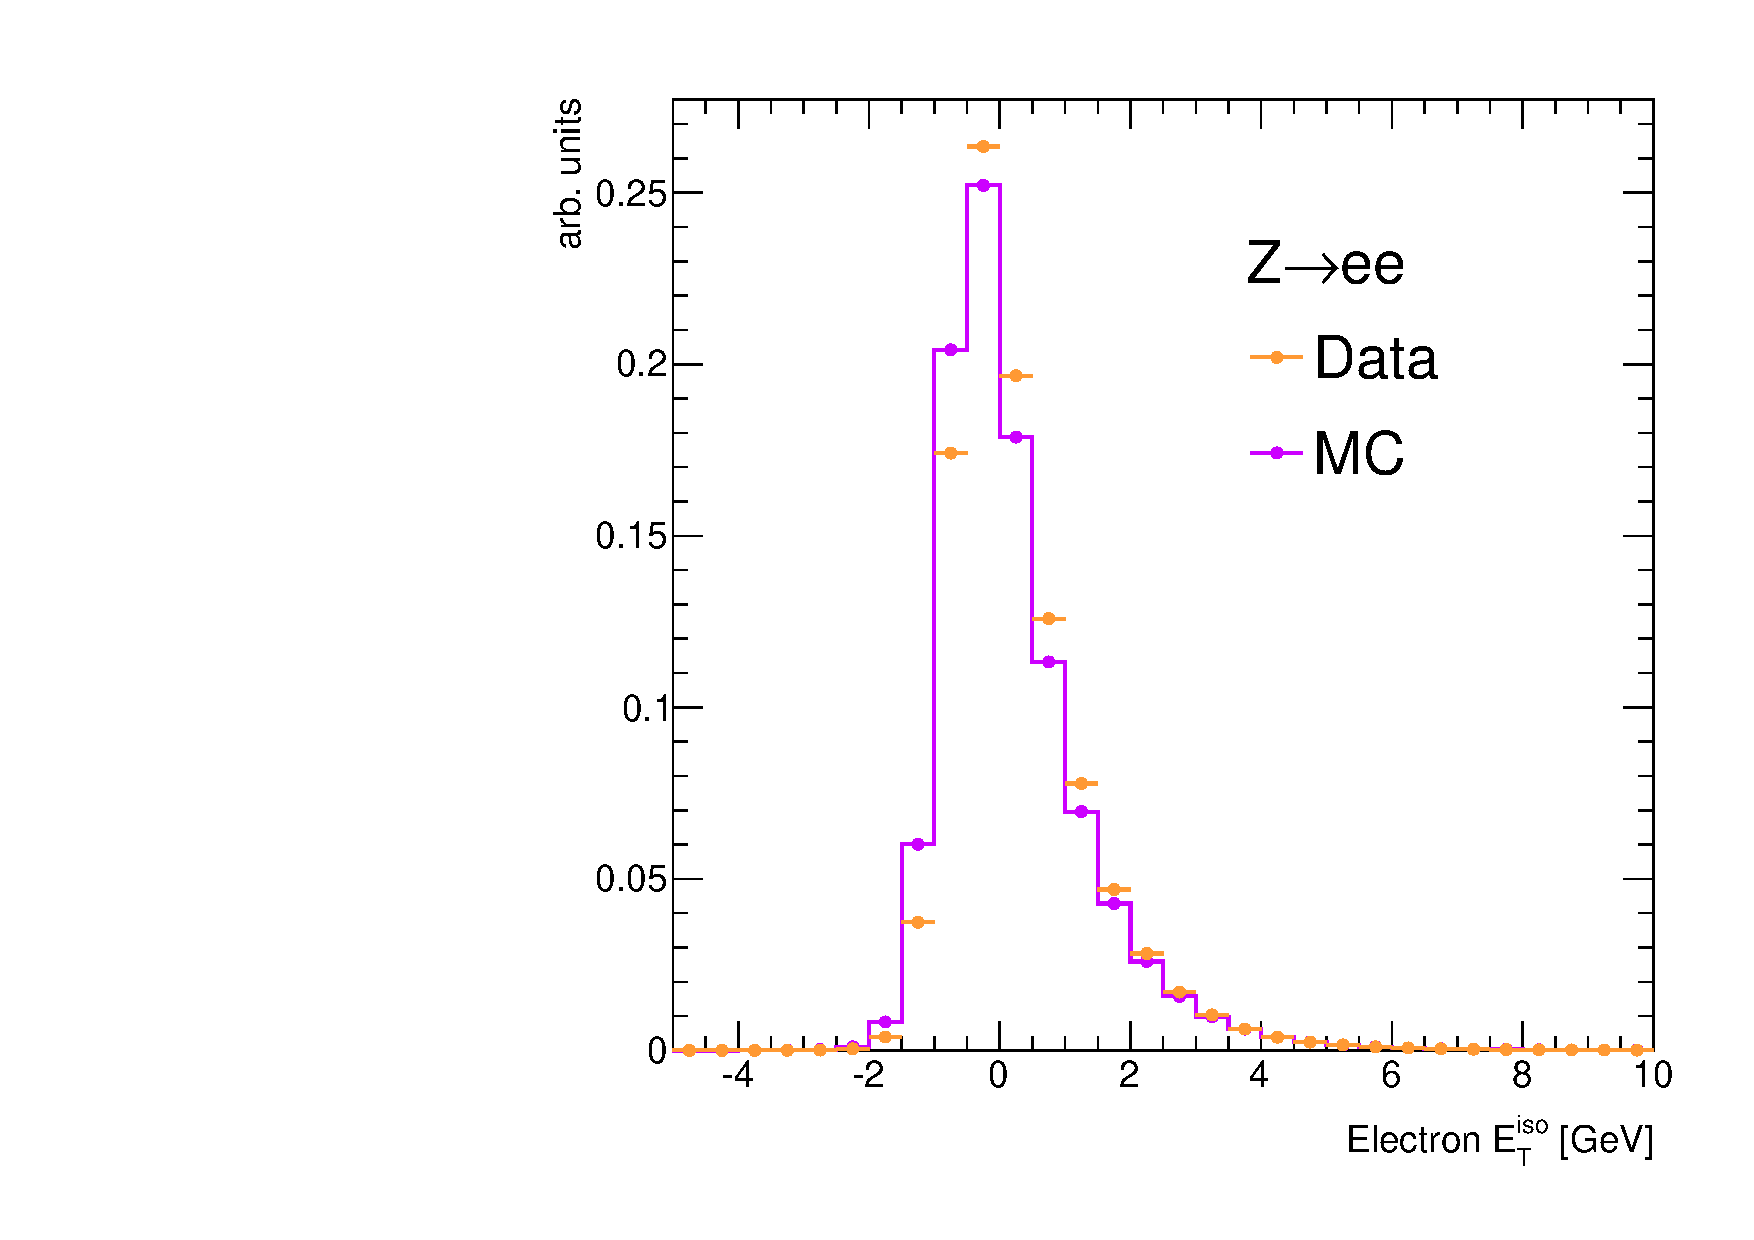
\includegraphics[width=0.49\textwidth]{electron_iso_Zee_raw}
  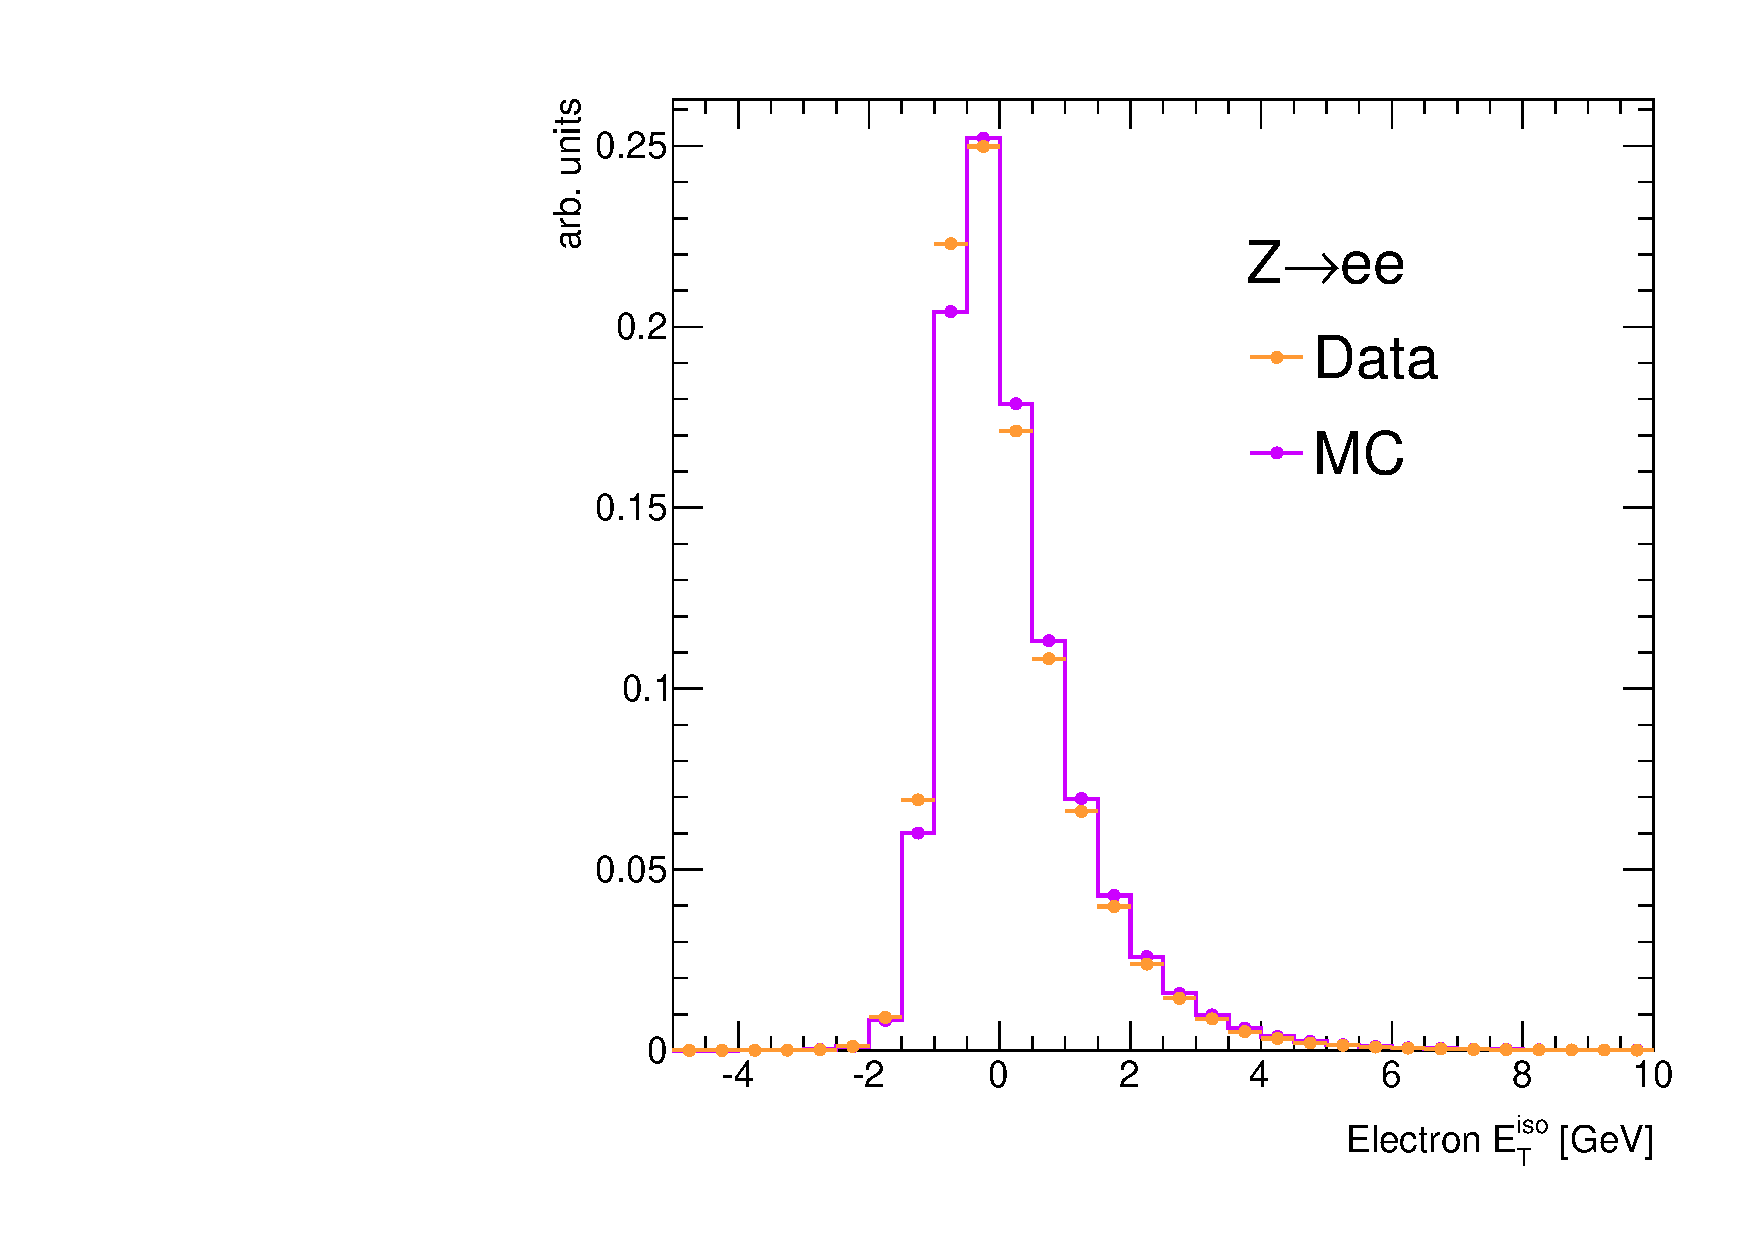
\includegraphics[width=0.49\textwidth]{electron_iso_Zee_corr}
  \caption{Comparacion datos/MC de la distribucion de {\etiso} de electrones provenientes de
    eventos {\Zee} (izquierda) y la correspondiente distribucion despues de aplicar la correccion
    por el {\pt} (derecha).}
  \label{fig:isolation_wandwo_correction}
\end{figure}

Para respaldar la estrategia de derivar el modelo de aislamiento de los fotones de
electrones se realizaron varios estudis. Una validacion importante del metodo consistio
en comparar la distribucion de {\etiso} de electrones provenientes de {\Zee} con la
El decaimiento radiativo del $Z$ provee un fuente de fotones puros. Los eventos se
seleccionaron requiriendo el siguiente conjunto de cortes, despues de la pre-seleccion:

\begin{itemize}\itemsep0.1cm
\item[-] Trigger: \texttt{EF\_2e12Tvhi\_loose1} $\parallel$ \texttt{EF\_e24vhi\_medium1} $\parallel$ \texttt{EF\_e60\_medium1}.
\item[-] Un foton \emph{tight} aislado con $\pt>25 \gev$.
\item[-] Dos electrones \emph{medium}, aislados, con carga opuesta, y con $\pt>50 \gev$ y $\pt>25 \gev$
\item[-] $\Delta R(\gamma,l)>0.7$
\item[-] \MET\ $<40\gev$
\item[-] $40\gev<m_{ee}<85\gev$
\item[-] $70\gev<m_{ee\gamma}<100\gev$
\end{itemize}

En la \cref{fig:photon_electron_iso} se presenta una comparacion entre
el modelo de fotones reaeles de decaimientos radiativos del $Z$ y electrones
de {\Zee}. El grafico a la derecha es obtenido despues de remover la dependencia
con el {\pt} con el factor de correccion como se describio anteriormente.
Puede verse de la {\fig} el buen acuerdo entre las distribuciones de {\etiso}
de fotones y electrones, en particular despues de aplicar la correcion, dando
confianza en la extrapolacion de usar electrones para modelar los fotones.
%% Vale la pena nota que el espectro de {\pt} de fotones tan bajo en estos
%% procesos (ver {\fig} \ref{fig:zllg_pt}) as compared to the generally broader electron \pt\ spectrum from Z decay. %of the electrons (see {\fig} \ref{fig:zeeg_pt}). \tosolve{add this last plot}

\begin{figure}[h]
  \begin{center}
    \includegraphics[width=0.49\textwidth]{figures/ph_el_data_raw}
    \includegraphics[width=0.49\textwidth]{figures/ph_el_correction}
    \caption{Comparison of isolation distributions  for real photons from radiative
      Z decays and electrons from \Zee\ before (left) and after the \pt\ correction
      is applied (right)}
    \label{fig:photon_electron_iso}
  \end{center}
\end{figure}

\begin{figure}[h]
  \begin{center}
    \includegraphics[width=0.49\textwidth]{figures/pt_sig_templates}
    \caption{Espectro del impulso transverso de fotones provenientes de decaimientos
      radiativos del Z, en datos.}
    \label{fig:zllg_pt}
  \end{center}
\end{figure}

Para estudiar el efecto To study the effect on the electron isolation template obtained from \Zee\ when using different
event topologies and kinematical regions, we present in \cref{fig:_electron_iso_HT},
the distributions for the case of different hadronic activity using a cut in \HT\ from simulations
on the left plot and from data \Zee\ on the right plot. As expected the electron template gets harder
and broader with \HT.  Unfortunately, the lack of statistic prevents us to apply a harder cut in \HT.
In any case, this effect will be consider as a possible source of systematic uncertainty.

\begin{figure}[h]
  \begin{center}
    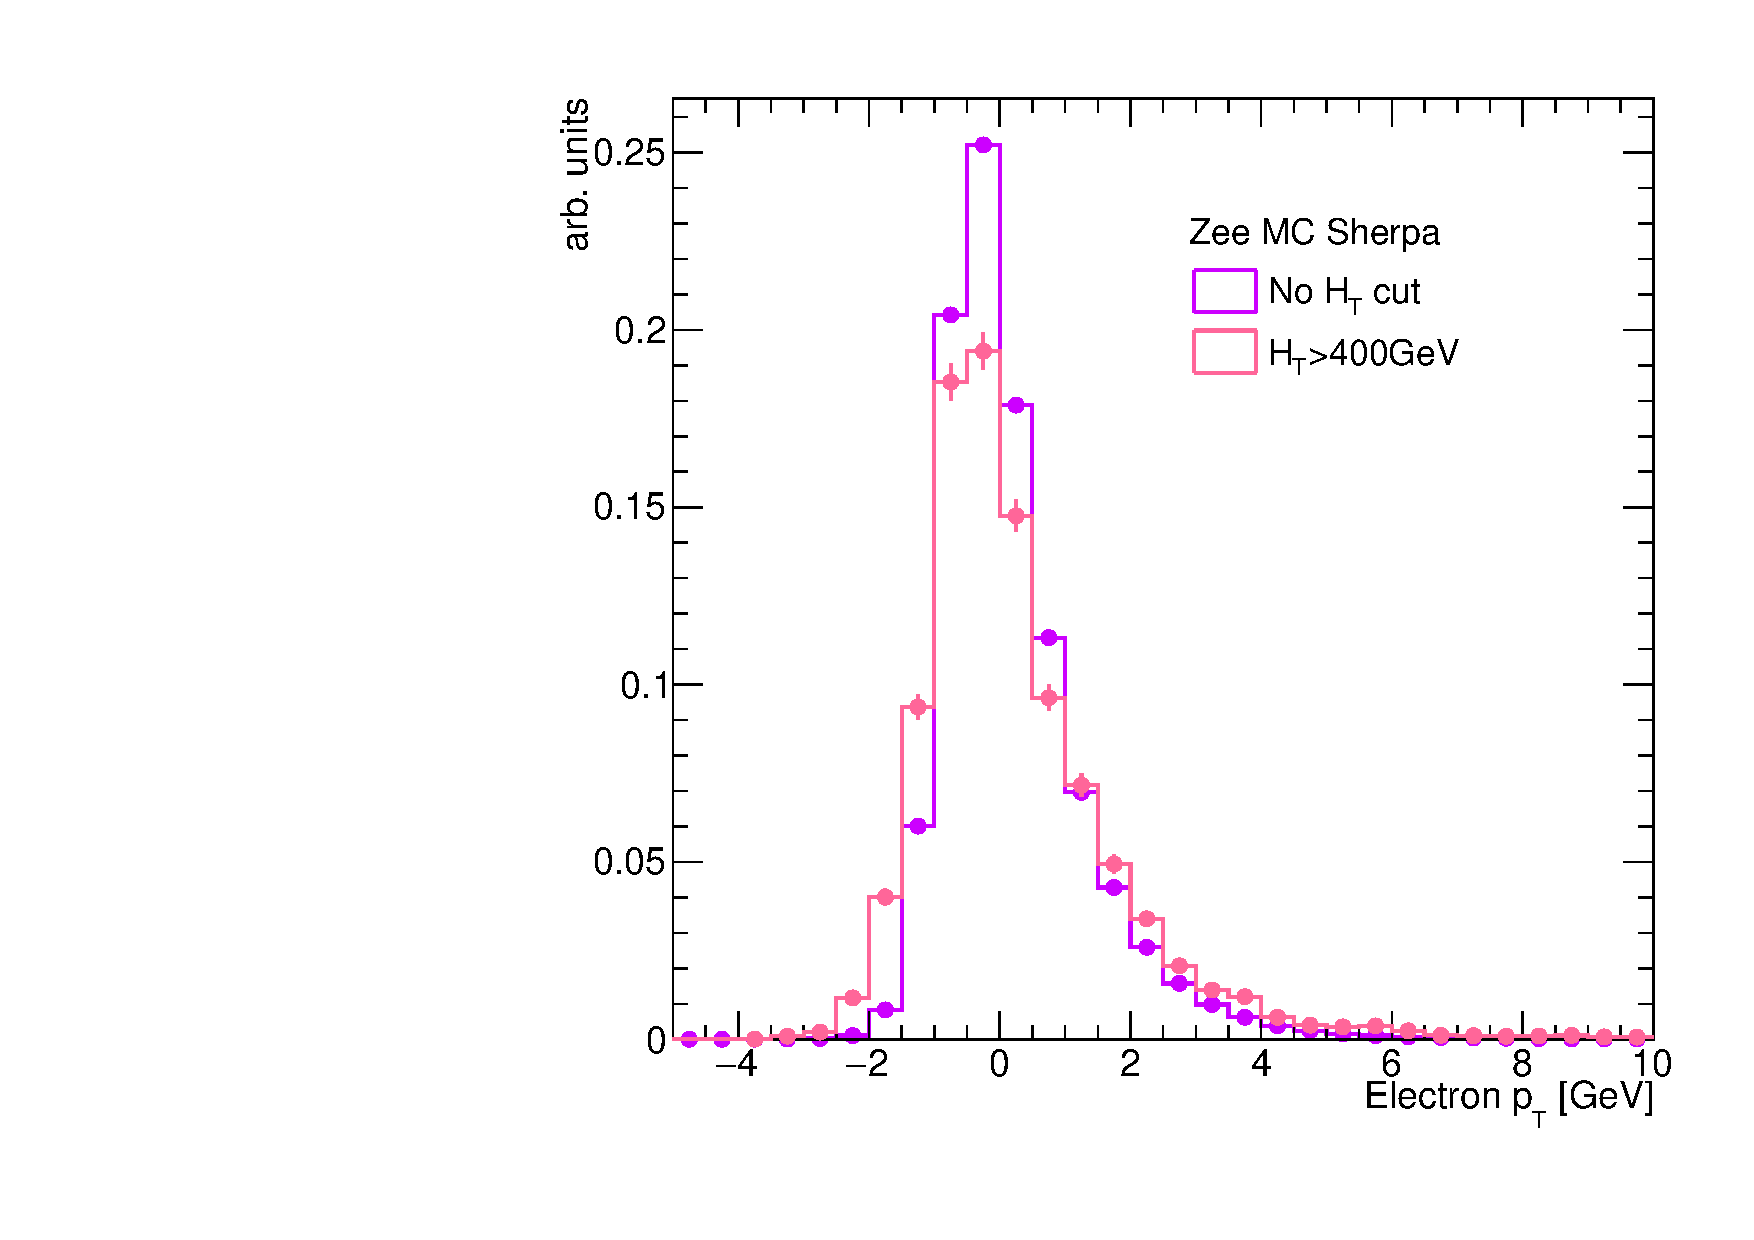
\includegraphics[width=0.49\textwidth]{figures/electron_iso_ZeeHMC_corr}
    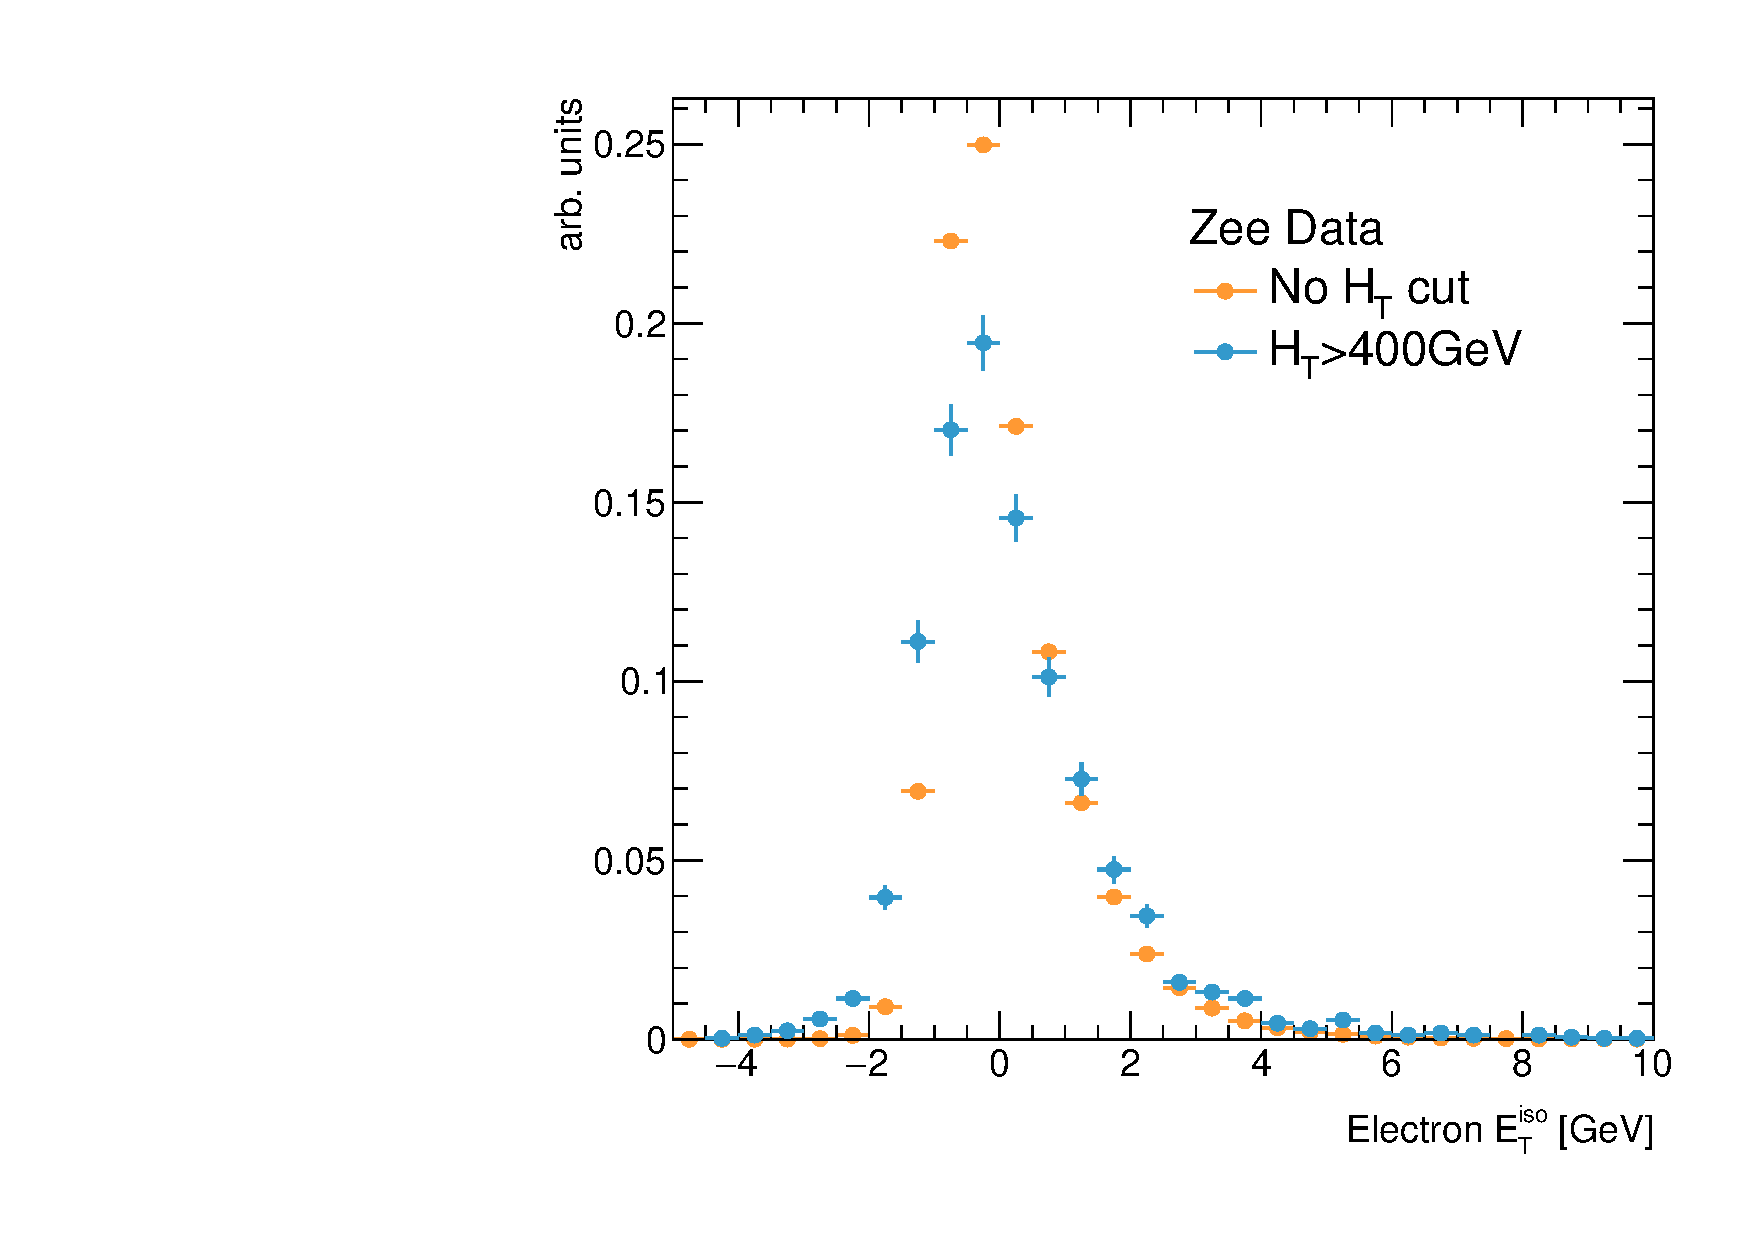
\includegraphics[width=0.49\textwidth]{figures/electron_iso_ZeeH_corr}
    \caption{Electron isolation dependency on \HT\ from MC (left) and data (right) \Zee}
    \label{fig:_electron_iso_HT}
  \end{center}
\end{figure}

\subsection{Modelo de fondo} \label{sec:jfake_bkg_template}

El modelo de fondo fue derivado de los datos, en eventos
que pasan todos los criterios de identificacion salvo los
criterios de identificacion \emph{tight} de fotones. La
muestra de pseudo-fotones

%% The background template was derived from the data, in events passing all signal requirements
%% but the tight photon ID cuts. The pseudo-photon sample selected this way should present an
%% isolation profile similar to that for the signal photons, allowing a low signal contamination
%% and high statistics. A dedicated study was done in MC to find the best set of tight ID cuts
%% to be reversed, in order to best model the expected isolation distribution for true hadronic fakes in the SR.
%% This is shown in {\fig} \ref{fig:jetfake_mc_data}, compared to the pseudo-photon sample in MC and data,
%% for two different ID definitions.
%% The loose-non-tight photons (LnT) are required to pass the loose ID, but fail at least one of
%% the tight cuts afterwards \footnote{For a detailed description of the photon ID variables
%%   please refer to \cite{ATLAS-CONF-2012-123}}. Despite of the larger statistics of the sample, it is clear that it
%% fails to model the background both in data and in the MC itself. A much better agreement is obtained for the loose'-non-tight (L'nT)
%% selection, in which the photons are requested to pass all the tight cuts but (at least) one on the narrow strips
%% variables ($F_\text{side}$, $w_{s3}$, $E_\text{ratio}$, $\Delta E$).
%% These variables are constructed with just a few central strips around the photon direction, and so are expected to be more
%% uncorrelated with the photon isolation, as it excludes the central cells to account for the photon self-energy
%% and covers a much wider region in space. This way, the pseudo-photon template mimics the tight photon shape and
%% allows the extrapolation to the signal region.

\begin{figure}[h]
  \begin{center}
    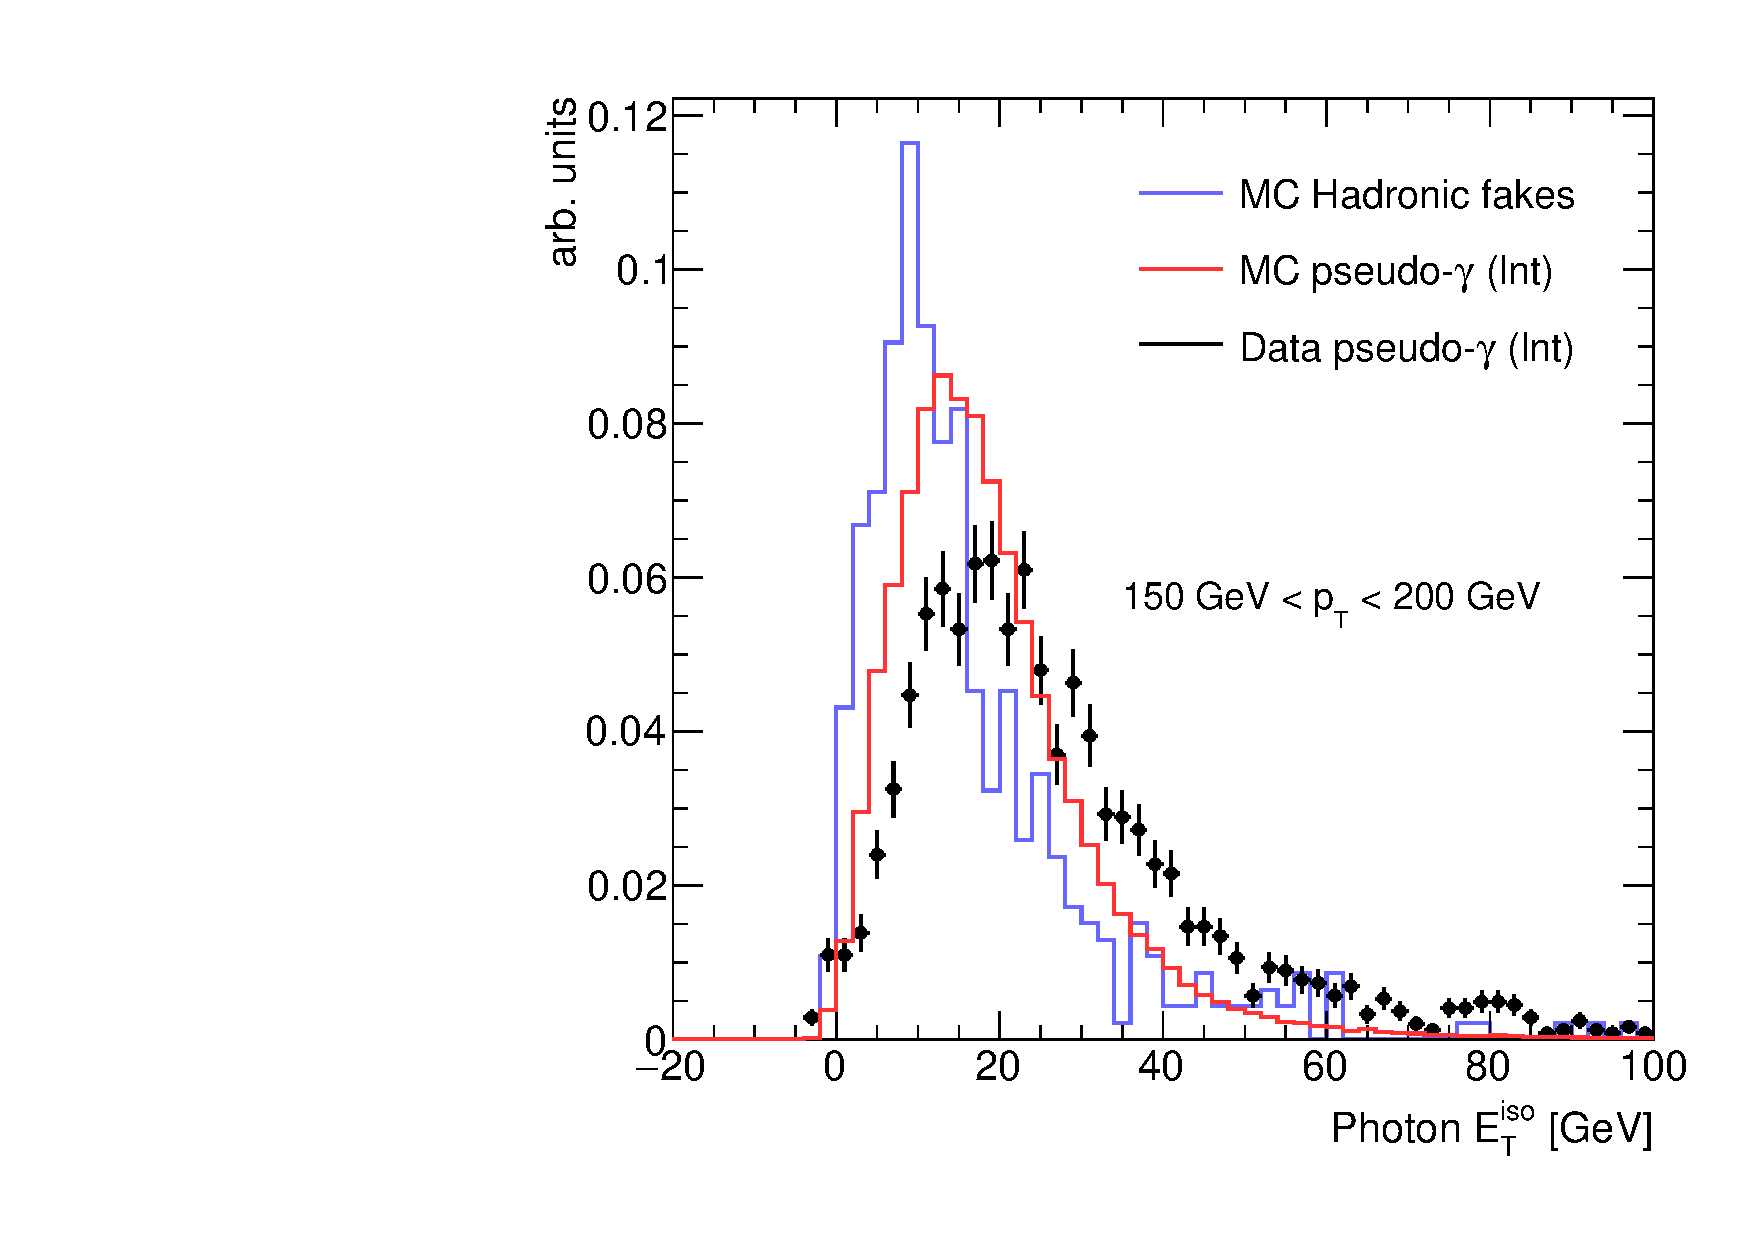
\includegraphics[width=0.49\textwidth]{figures/bkg_mc_pseudo_data_SR_l_ptbin}
    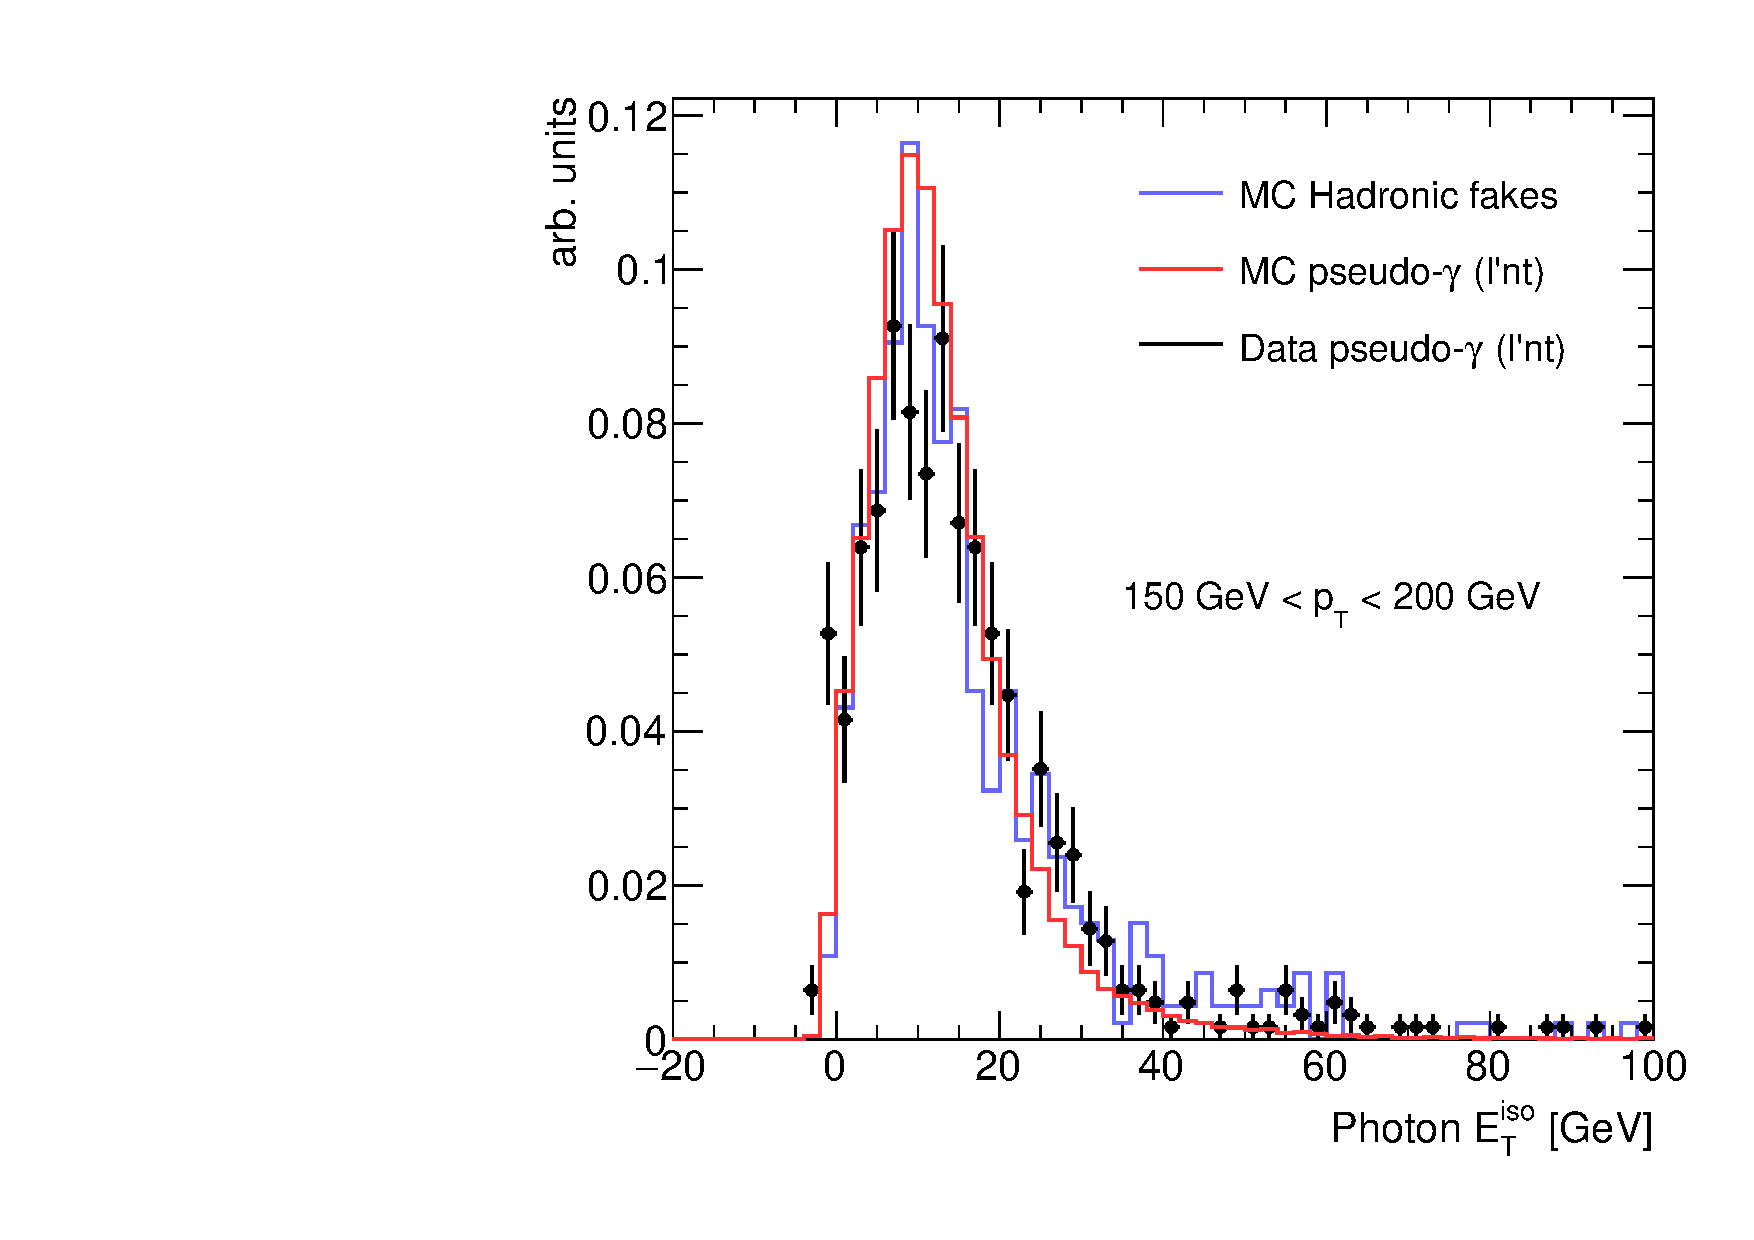
\includegraphics[width=0.49\textwidth]{figures/bkg_mc_pseudo_data_SR_lp_ptbin}
    \caption{Isolation distribution for truth MC photon fakes from hadronic decays, compared to pseudo-photon
      sample obtained in MC for background, obtained in the (right) nominal and (left) loose signal regions.}
  \label{fig:jetfake_mc_data}
  \end{center}
\end{figure}

%% Evenmore, as seen in {\fig} \ref{fig:jetfake_pseudo_data_pt}, the \pt\ spectrum of the L'nT photon candidates
%% better reproduce that expected for tight photons. No further \pt-reweighting is needed in this case.
%% Similarly, {\fig} \ref{fig:jetfake_pseudo_data_BE} shows the only slight shape difference for pseudo-photons
%% in the barrel and endcap regions.

%% Particularly for fake events, the extrapolation from the region used to derive the faking probability ratio and
%% the respective signal region might suffer from different topology and kinematics of the events in each case.
%% For this reason, the control region selection to derive the templates is kept close to the SR, as listed in {\tab} \ref{tab:cr_jetfake}.
%% An orthogonality requirement is placed on \MET ($50-150\gev$) and some SR cuts are loosened to retain statistics.
%% As expected, however, the larger the jet activity around the harder the photon isolation in the event. So the
%% \HT\ requirements can not be loosened much. This can be clearly observed in {\fig} \ref{fig:jetfake_pseudo_data_LR_VR},
%% for a loose (CRFJL: $>200 \gev$) and tight (CRFJ: $>600 \gev$) \HT\ selection. The latter is therefore used to
%% perform the combined fit and to compute the jet fake factor, as discussed in the next section.

\begin{table}[h!]
  \centering
  \caption{Control region definition for jet fake estimation.} %%The final estimate in SR for this background is obtained by weighting the yields in the control region (CRJ), by the
  %%$f_{j\to\gamma}$ fake factor derived in the CRFJ region. The numeric suffix indicates (when present) the SR associated to each region (SR2 or SR3).}
  \begin{tabular}{rcc}
    \hline \hline
    %%  & CRJ2(3) & CRFJ & CRFJL \\
    %% \hline %\hline
    %% $\pt(\text{pseudo}-\gamma_1)$ (\gev) $>$ &  125         &   125 & 125 \\
    %% N leptons                                &   0          &     0 &     0     \\
    %% \met (\gev)                              & $>$150 (300) &  $50<\met<150$        & $50<\met<150$      \\
    %% N jets $\ge$                             &    4 (2)     &   2       &   2     \\
    %% $\pt(j_1,2)$  (\gev)  $>$                & 100  (80)    &   100     & 100   \\
    %% $\dphijm >$                              & 0.4          &   0.4      &  0.4    \\
    %% \HT (\gev) $>$                           & - (800)      &   600    &  200   \\


         & CRFJ & CRFJL \\
    \hline %\hline
    $\pt(\text{pseudo}-\gamma_1)$ (\gev) $>$ &    125 & 125 \\
    N leptons                                &      0 &     0     \\
    \met (\gev)                              &   $50<\met<150$        & $50<\met<150$      \\
    N jets $\ge$                             &    2       &   2     \\
    $\pt(j_1,2)$  (\gev)  $>$                &    100     & 100   \\
    $\dphijm >$                              &    0.4      &  0.4    \\
    \HT (\gev) $>$                           &    600    &  200   \\
\hline \hline
  \end{tabular}
\label{tab:cr_jetfake}
\end{table}


\begin{figure}[h]
  \begin{center}
    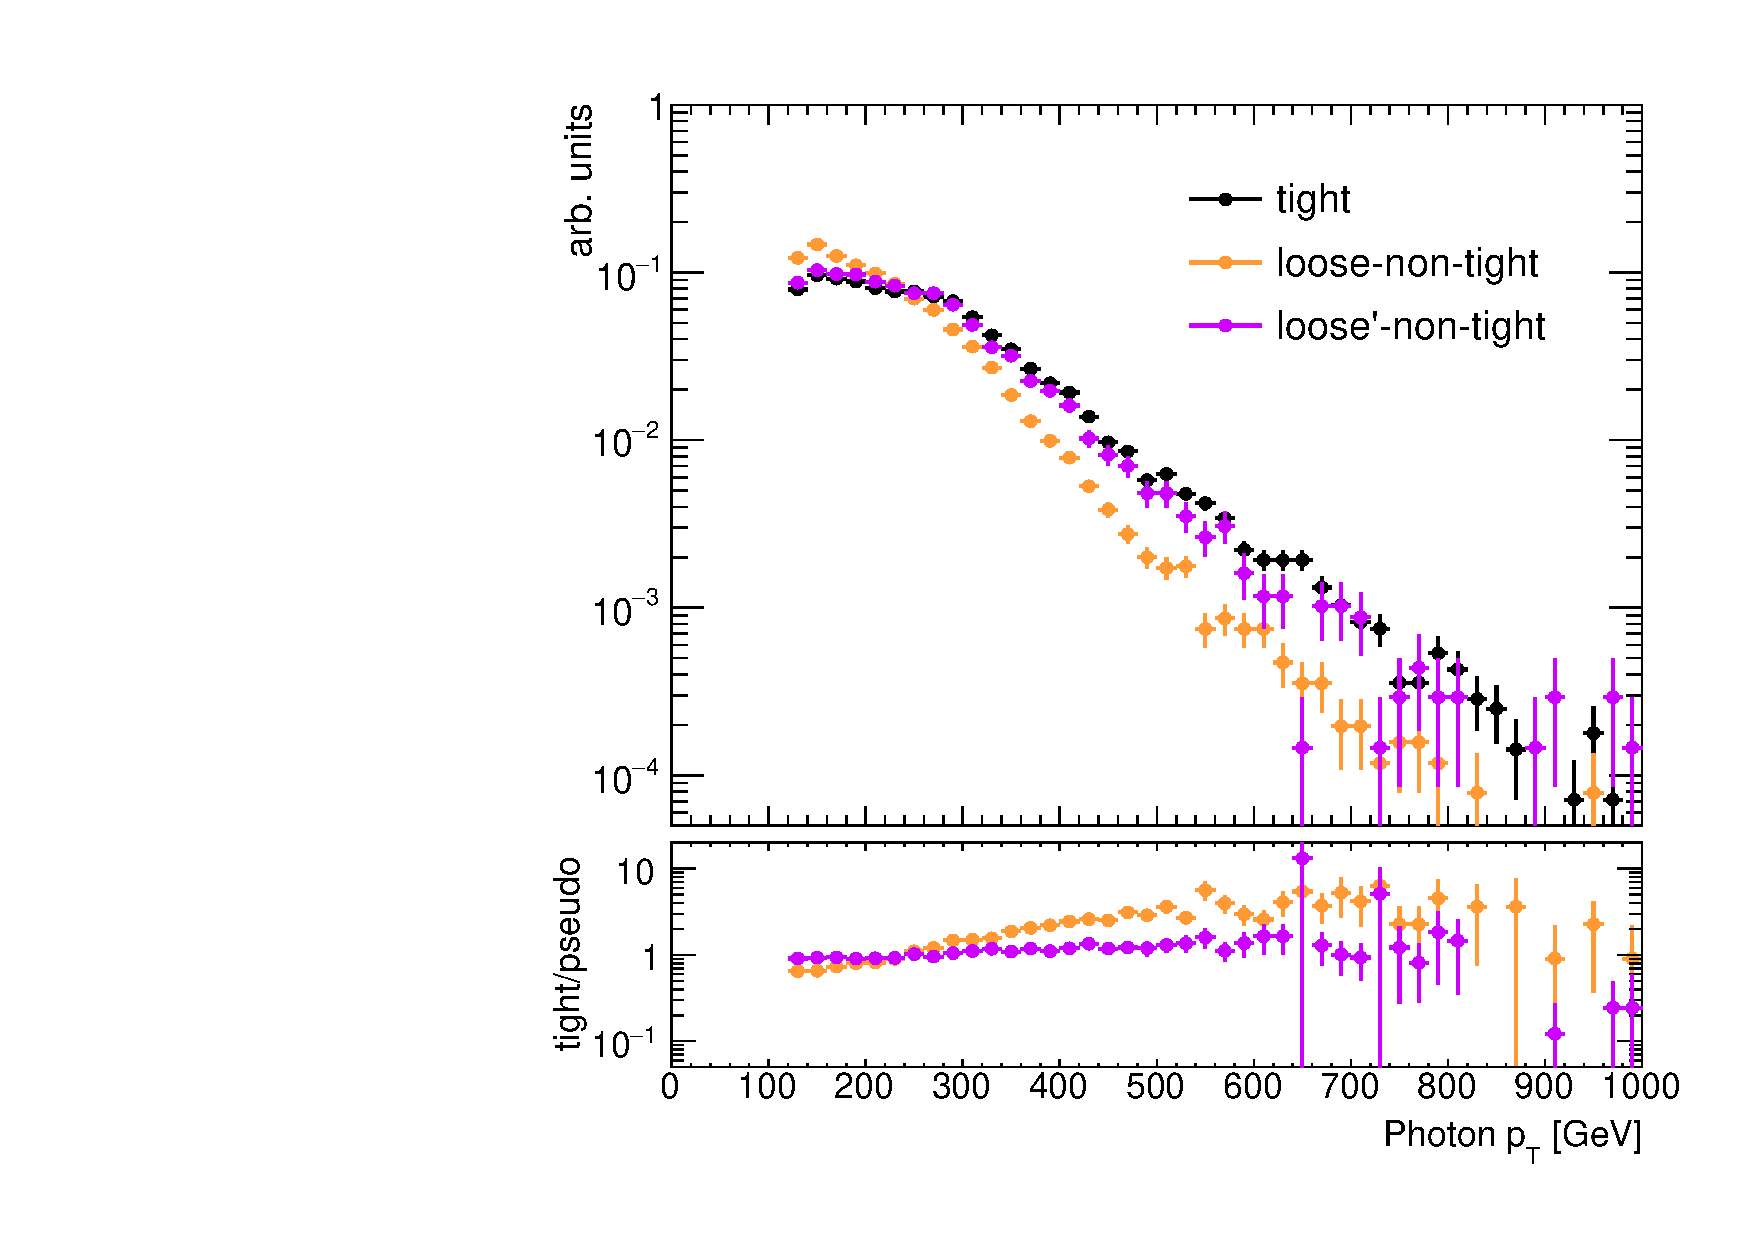
\includegraphics[width=0.49\textwidth]{figures/bkg_data_pseudo_tight_data_VR}
    %% \caption{Distribución del {\pt} del foton para candidadtos
    %%   \emph{tight and pseudo-photon candidates, after full CRFJ selection.}
  \label{fig:jetfake_pseudo_data_pt}
  \end{center}
\end{figure}

\begin{figure}[h]
  \begin{center}
    \includegraphics[width=0.49\textwidth]{figures/bkg_pseudo_data_SREB_l}
    \includegraphics[width=0.49\textwidth]{figures/bkg_pseudo_data_SREB_lp}
    %% \caption{Isolation templates for loose-non-tight (left) and loose'-non-tight (right) pseudo-photon data,
    %%   after full CRFJ selection, in barrel and endcap regions.}
  \label{fig:jetfake_pseudo_data_BE}
  \end{center}
\end{figure}

\begin{figure}[h]
  \begin{center}
    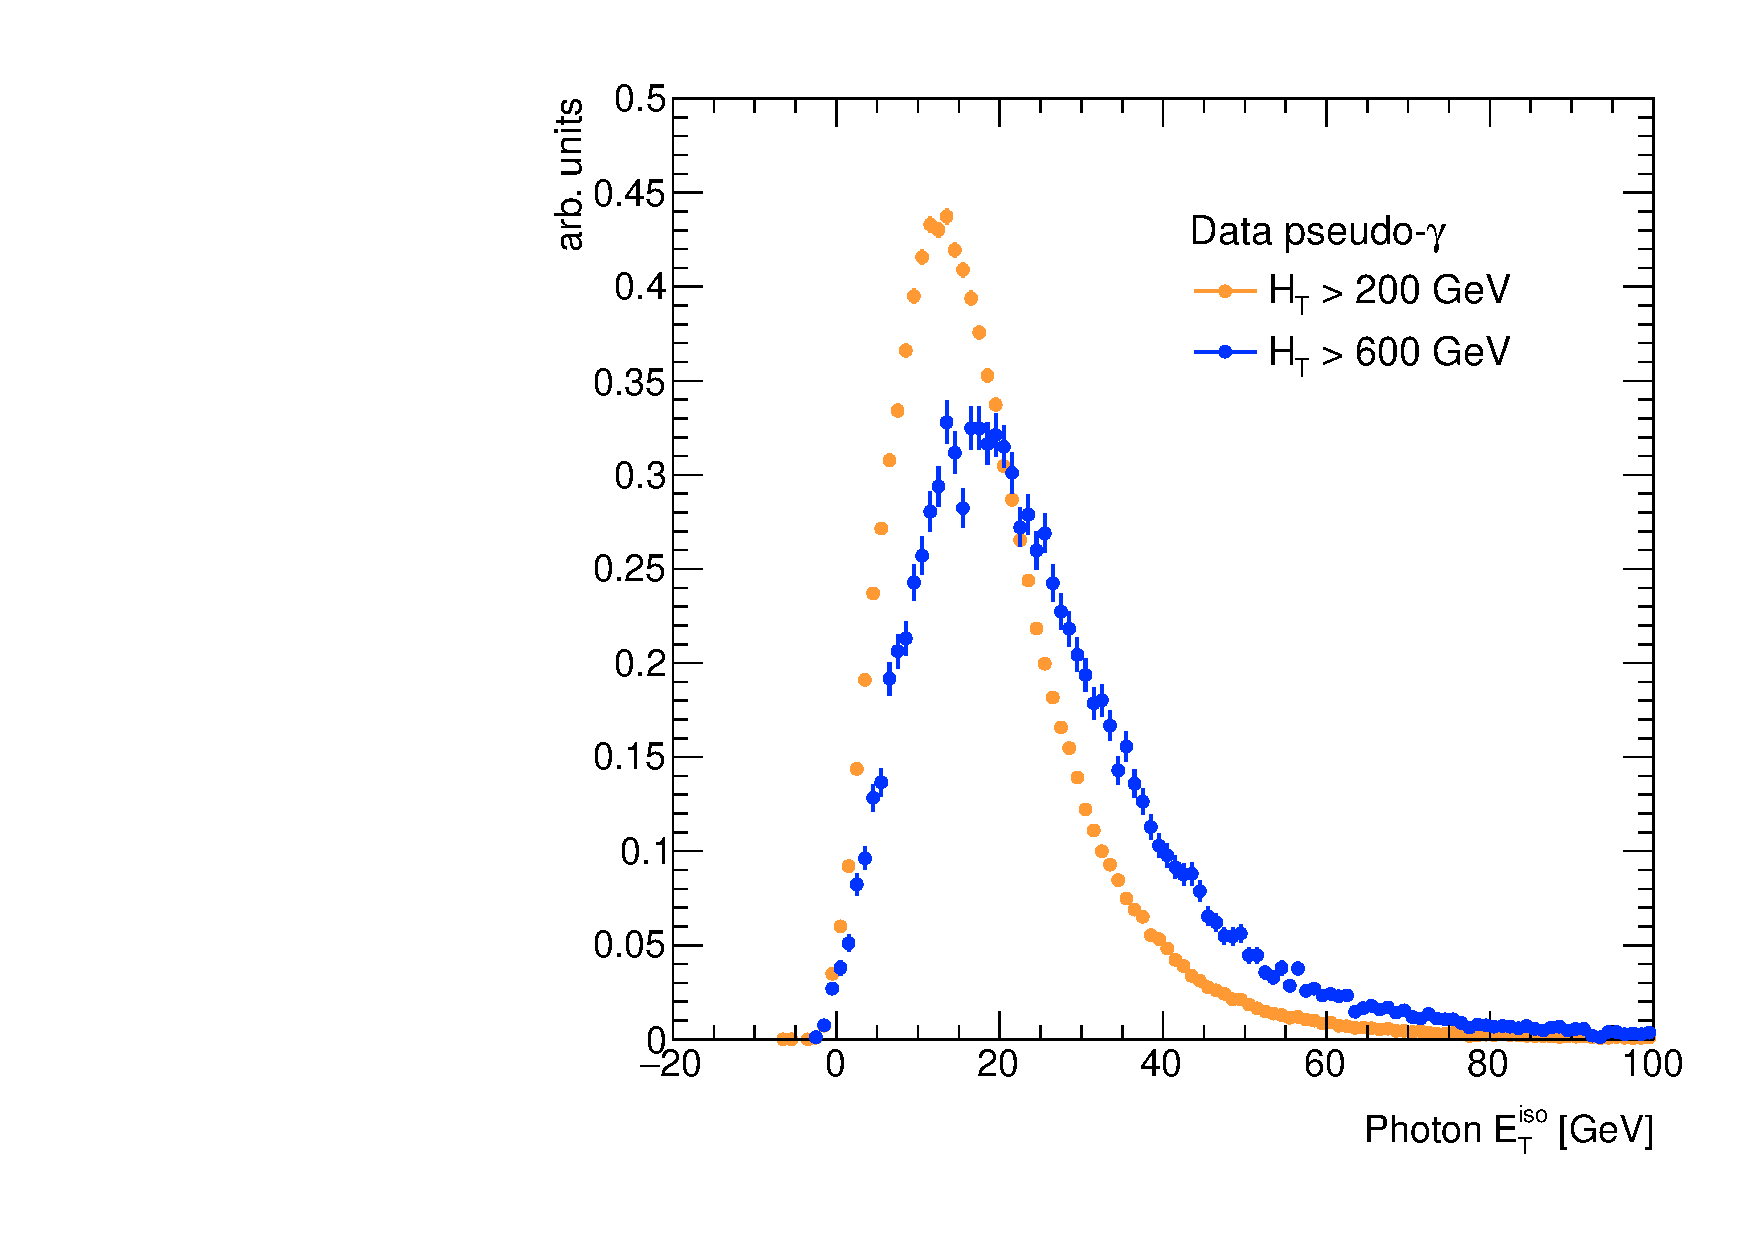
\includegraphics[width=0.49\textwidth]{figures/bkg_pseudo_data_SR_VR_l}
    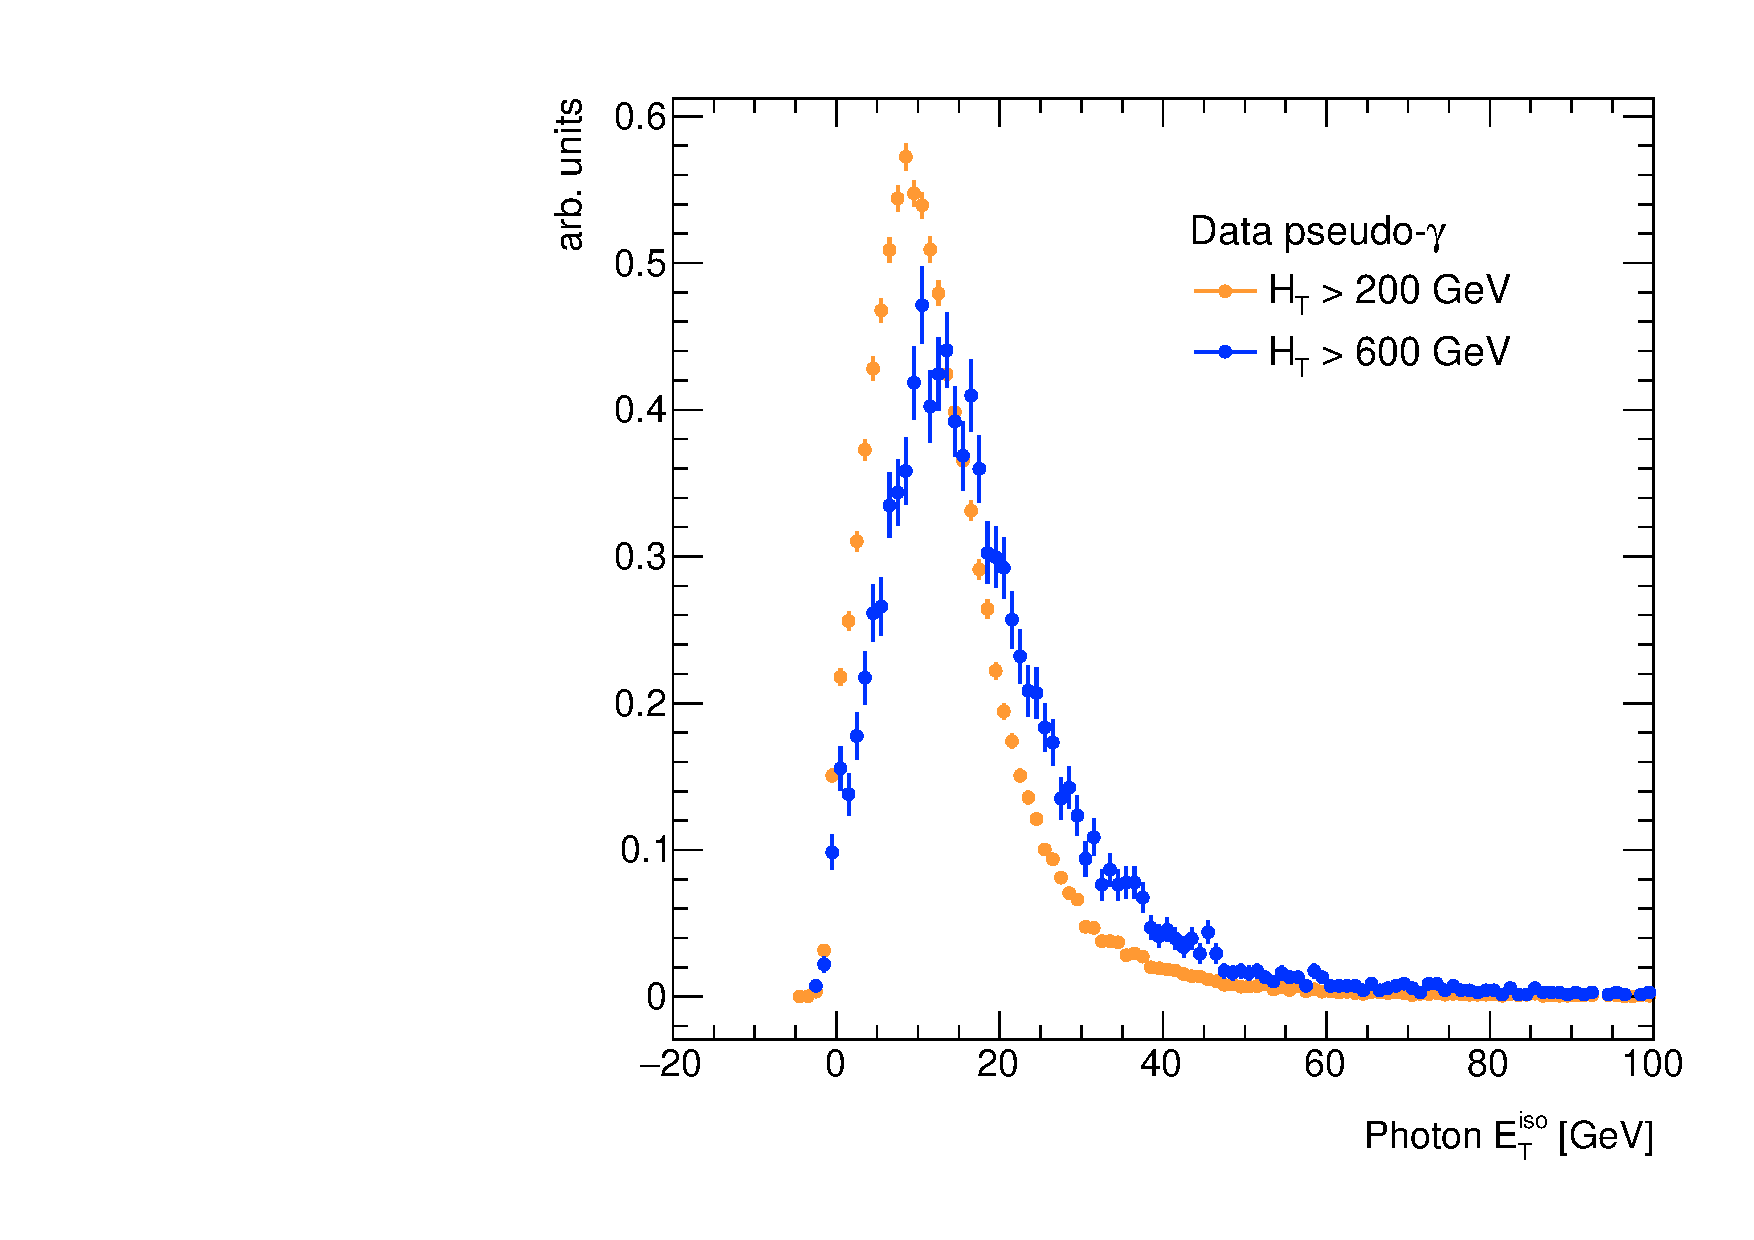
\includegraphics[width=0.49\textwidth]{figures/bkg_pseudo_data_SR_VR_lp}
    %% \caption{Isolation templates for loose-non-tight (left) and loose'-non-tight (right) pseudo-photon data,
    %%   after signal-like selection with a  loose (CRFJL: $>200 \gev$) and tight (CRFJ: $>600 \gev$) \HT\ cut.}
  \label{fig:jetfake_pseudo_data_LR_VR}
  \end{center}
\end{figure}

Finally, the background template from loose'-non-tight photons in the CRFJ region is found
to be well described by a Crystall Ball function. The data distribution and the fitted profile
is shown in \cref{fig:jetfake_sigbkg}. The parametrized template is used in the combined
fit to tight photon data to derive the jet fake rate.

%% \begin{figure}[h]
%%   \begin{center}
%%   \includegraphics[width=0.49\textwidth]{iso_fit_bkg_wpars}
%%   \caption{Fit to the observed isolation template for  loose'-non-tight pseudo-photon data in the VR.}
%%   \end{center}
%%   \label{fig:jetfake_bkg_template_fit}
%% \end{figure}

\subsection{Ajuste combinado y estimacion del fondo} \label{sec:jet_fake_results}

A template fit to both signal and background distributions is then used to model the shape of the photon isolation
for each contribution, as shown in \cref{fig:jetfake_sigbkg}, together with the fitted parameters.
%The corresponding $\chi^2$/dof are 2.4 and 8.8 for signal and background templates with 240 points.

La distribucion de {\etiso} para todos los eventos que pasan los criterios
de seleccion de la region relajada (CRFJ) es ajustada a una combinacion
lineal de los modelos de senal y fondo. El ajuste combinado y cada componente
de la distribucion pueden verse en \cref{fig:jetfake_combfit}.
Los parametros son inicializados con los valores extraidos de los ajustes
individuales a la senal y el fondo, y se los permite variar dentro de su
incerteza
%As this fit is the source of the biggest systematic uncertainty the range of the parameters is then extend to two times the
%individual fit uncertainties to compute the systematic of the method.

Para estimar la incerteza sistematica, el ajuste combinado es realizado
sin ningun constrarin en los parametros. La incerteza obtenida es del
50\% del valor de$f_{j\to\gamma}$, lo suficientemente grande para contener
cualquier potencial mismodelado de los templates.

%The fitted parameters for the signal, background and combined fits are tabulated in \Tab \ref{tab:jetfake_fit_pars}.
Los parametros estimados del ajuste combinado estan tabulados en la
\cref{tab:jetfake_fit_pars}.

El numero de fotones total (N$_\text{tot}^\text{iso}$) y fake (N$_{j\to\gamma}^\text{iso}$)
esperados en la region de control es obtenido integrando
las componentes de fondo y total del ajuste combinado sobre todo el rango
$\etiso<5\gev$, respectivamente:

\begin{itemize}
\item[] N$_{j\to\gamma}= 24143 \pm 56$

\item[] N$_\text{tot}= 281812 \pm 533$
\end{itemize}

La fraccion $f_{j\to \gamma}$ es obtenida simplemente como el cociente
en la \cref{eq:jfake_formula}:

\begin{itemize}
\item[] $f_{j\to\gamma} = 0.0857 \pm 0.0002 \stat \pm 0.04 \;\syst$
\end{itemize}

\begin{figure}[h]
  \begin{center}
  \includegraphics[width=0.49\textwidth]{figures/iso_fit_sig_wpars}  \hfill
  \includegraphics[width=0.49\textwidth]{figures/iso_fit_bkg_wpars}
  \caption{Ajuste a las distribuciones de {\etiso} de senal
    (izquierda) y fondo (derecha) (right) en la region
    de control CRFJ.}
  \label{fig:jetfake_sigbkg}
  \end{center}
\end{figure}

\begin{figure}[h]
  \begin{center}
  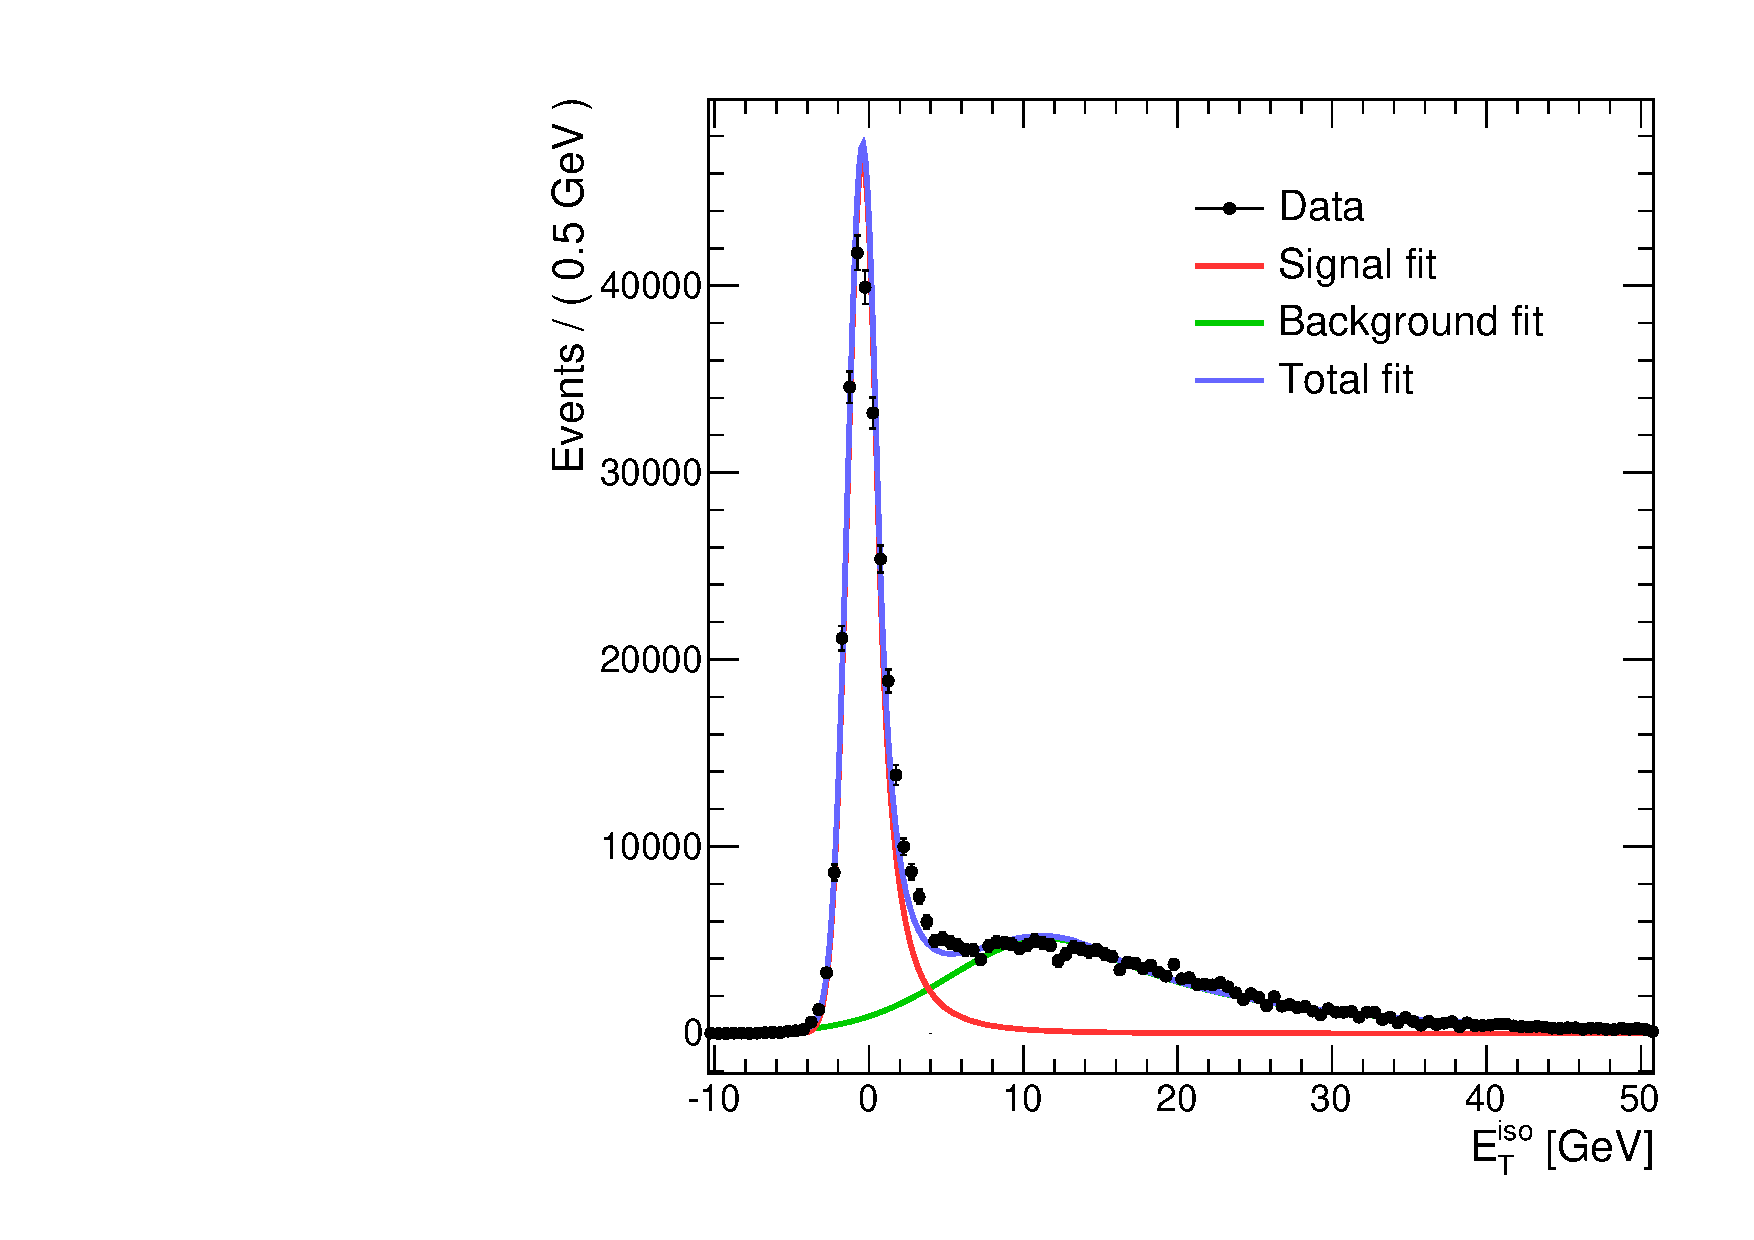
\includegraphics[width=0.49\textwidth]{figures/iso_fit_sarange}
  \caption{Ajuste combinado a la distribucion de {\etiso}
    para los pseudo-fotones que pasan la selección de la región
    de control CRFJ (ver texto para detalles).}
  \label{fig:jetfake_combfit}
  \end{center}
\end{figure}

\begin{table}[h!]
  \centering
  \caption{Fit parameters results from the combined fit to the isolation distribution of pseudo-photon data in CRFJ. Both signal and background were found to be well described by a Crystall Ball function.}
  \begin{tabular}{l l}
     Parameter &  Fit result \\
     \hline
     \verb|bkg_cb_alpha| & $-0.5932 \pm 0.0003$ \\
     \verb|bkg_cb_mean|  & $11.4897 \pm 0.0009 \GeV$ \\
     \verb|bkg_cb_n|     & $9.33 \pm 0.03$ \\
     \verb|bkg_cb_sigma| & $6.2862 \pm 0.0008 \GeV$ \\
     \verb|bkg_yield|    & $216579 \pm 500$ \\
     \hline
     \verb|sig_cb_alpha| & $-1.0460 \pm 0.0001$ \\
     \verb|sig_cb_mean|  & $-0.4175 \pm 0.003 \GeV$ \\
     \verb|sig_cb_n|     & $3.6675 \pm 0.0007$ \\
     \verb|sig_cb_sigma| & $0.9819 \pm 0.0001$ \\
     \verb|sig_yield|    & $2654337 \pm 546$ \\
     \hline
   \end{tabular}
    \label{tab:jetfake_fit_pars}
\end{table}


The number of jets faking photons can be estimated now using the fraction $f_{j\to\gam}$ as,

\begin{equation}\label{eq:njfakes}
  N_\text{fakes} = f_{j\to\gam} \times N_\text{tight}
\end{equation}

To keep the analysis blinded, we parametrize the number of fakes as function of \met, as shown in \cref{fig:jetfake_nfakes_met}, using an exponential
function $N_\text{fakes} = \exp(A+B \, \met)$. The values of the $A$ and $B$ parameters obtained from the fit are shown in table \cref{tab:exppars}.

\begin{table}[h!]
  \centering
  \caption{Fit parameters results from the fit to the $N_\text{fakes}$ distribution as a function of \met with an exponential function $\exp(A+B\, \met)$.}
  \begin{tabular}{crr}
    \hline
    Parameter &  SR2 & SR3 \\
     \hline
     A & $3.87 \pm 1.25$  &  $1.80 \pm 0.98$ \\
     B &  $-0.054 \pm 0.018$  & $-0.047 \pm 0,014$ \\
     \hline
  \end{tabular}
  \label{tab:exppars}
\end{table}


The final background contamination expected from jets faking photons is obtained integrating the $N_\text{fakes}$ parametrization over the \met region
of each SR:

\begin{align}
  N_\text{fakes}^\text{SR2} &= \int_{200}^{\infty} N_\text{fakes}(\met) \, d\met = 0.01 \pm 0.02 \\
  N_\text{fakes}^\text{SR3} &= \int_{300}^{\infty} N_\text{fakes}(\met) \, d\met = 0.0001 \pm 0.0001
\end{align}


\begin{figure}[h]
  \centering
  \includegraphics[width=0.49\textwidth]{figures/nfakes_SR2}  \hfill
  \includegraphics[width=0.49\textwidth]{figures/nfakes_SR3}
  \caption{Parametrización del número de jets mal identificados como
    función de {\met}.}
  \label{fig:jetfake_nfakes_met}
\end{figure}

El fondo de jet fakes es estimdo similarmente en las regiones de control
y validacion definidas en la \cref{tab:sr2,tab:sr3}, pesando
el numero de eventos observado en cada cosa por el factor $f_{j\to\gamma}$. % factor above as in \Eq \ref{eq:njfakes}.


%% The final background contamination expected from jets faking photons is obtained by weighting the number of events observed in data,
%% after the otherwise full tight SR selections detailed in sec \ref{sec:signal_regions} (i.e. only the photon identification requirement is reversed).


%% Indeed, no pseudo-photon event was ultimately observed after all CRJ selections. This leads to a
%% j$\to\gamma$ background estimate of $<0.07$ events. Consistently, MC studies have shown this
%% background to be small in the high \MET\ and \HT\ regimes on the final SRs. As seen in \Tab \ref{tab:mc_events_sr_phtype}, the
%% MC predicts a jet fake contamination of $0.10\pm 0.04$ and $0.02 \pm 0.02$ event for SR2 and SR3, respectively.
%% This supports the findings in the data, agreeing within the uncertainties. The final jet fake background yield is estimated as $N^\text{SR}_\text{jfakes} = 0.0^{+0.1}_{-0.0}$, which accommodates an extra $+0.03$ uncertainty from the comparison of the MC-data predictions.

%\tosolve{add check with MET-stepped predictions?}.


%In absence of observed events surviving the SR selection, a conservative estimate is computed under the assumption
%of one event in the pseudo photon sample for each signal region. It translates to a final yield of


%The final background contamination expected from jets faking photons was obtained by weighting the number of pseudo-photon events observed
%in data, after the otherwise full tight SR selections detailed in sec \ref{sec:signal_regions}. i.e. only the photon identification requirement is reversed.
%The results are summarized in \Tab \ref{tab:jetfake_yields}.
%
%\begin{table}[h!]
%  \centering
%  \caption{Number of misidentified jet events expected in the different signal regions. The unscaled number of pseudo-photons
%    is weighted by the $f/p$ ratio to get the final background yield from jet fakes in the three
%    analysis regions.}
%
%  \begin{tabular}{ccc}
%    \hline
%    \hline
%    Signal region & Unscaled & Weighted  \\
%    \hline
%%    SR1 & $4$ & $7.50$ \\
%    SR2 & $0$ & $0.00$ \\
%    SR3 & $0$ & $0.00$ \\
%    \hline
%    \hline
%  \end{tabular}
%  \label{tab:jetfake_yields}
%\end{table}

%\section{Regiones de Control}\label{sec:CRs}

%The control regions used in the analysis are listed in {\tab} \ref{tab:CRs} and depicted in {\fig} \ref{fig:CRVRSR}. There are 2 CRs associated with each SR. Each CR$_i$ (i=1,2,3) selection is designed to enhance the population of one of the main backgrounds in the associated SR$_i$ (QCD, W($\to \ell\nu$)/Z($\to \ell\ell$)+\g,
%\ttbar+\g). Any other contamination is either taken from MC (Dibosons, Z($\nu\nu$+jets/\g)) or estimated with the data-driven techniques described in sec \ref{sec:background_estimation}.
%The control regions used in the analysis are listed in {\tab} \ref{tab:CRs} and depicted in {\fig} \ref{fig:CRVRSR}.

%% There are three control regions (CR) associated with each SR,
%% designed to enhance the population of the expected %the main%
%% backgrounds in this analysis, {\wgam} (CRLW), {\ttgam} (CRLT)
%% and QCD {\gjet} (CRM) events. The selection details are summarised
%% in {\tab} \ref{tab:sr2} and \ref{tab:sr3}. Any other contamination
%% is either taken directly from MC (\ttgam) %, Dibosons, Z($\nu\nu$+jets/\gam))
%% or estimated with the data-driven techniques described in sec \ref{sec:background_estimation}.

%The contribution from QCD \gjet\ is modeled with the jet smearing method detailed in the sec \ref{sec:jetsmearing}, to emulate the fake \etmiss\ caused by the jet energy mismeasurement.
%% The final estimate for this background is obtained by normalizing the smeared events passing a dedicated selection (CRQ) defined
%% from the corresponding SR by reversing the \dphijm\ cut ($<0.2$) and removing the $R_{T}$ cuts. An intermediate \dphijm\ region between 0.2 and 0.4 is kept for validation purposes.
%% CRQ selects a sample of events with similar kinematics to the SR but enriched in QCD background events. The QCD multijets contamination in this region,
%% estimated with the ratio method explained in sec \ref{} is explicitly removed from the selected sample to avoid double counting in the global fit
%% described in sec \ref{sec:fitconfig}.
%% The final estimate for the prompt photon background is obtained by normalizing the Sherpa MC events passing a dedicated selection (CRM) defined
%% from the corresponding SR but at low {\met} ($< 50 \gev$). As expected,  CRM selects an enriched sample %of events with similar kinematics to the SR but enriched in
%% of QCD background events. The multijet contamination is independently estimated with the ratio method explained in sec \ref{sec:jetfakes}. %, is explicitly removed from the selected sample to avoid double counting in the global fit described in sec \ref{sec:fitconfig}
%% Some intermediate {\met} regions between 50 {\gev} and the SR cut are kept for validation purposes. Given the large jet multiplicty and \MET requirements in SR2 and SR3, respectively, the prompt photon background is
%% expected to be very small in both signal regions. However, its contribution is not negligible in the control and validation regions so it is important to get a good normalization estimate.


%CRLT and CRLW select respectively \ttbargam and \wlnugam events, by requiring a photon, a lepton, jets and \etmiss. A {\it b}-veto(tag) requirement is applied in CRLW(CRLT) to enrich the sample in \ttbargam and \wlnugam events.
% Both CRs use a looser \etmiss selection with respect to the SR value, as otherwise the control region suffers from lack of statistics.

%% The CRLW and CRLT selections aim for {\wgam} and {\ttgam} events, respectively,
%% by requiring a photon, a lepton, jets and \met. A $b$-jet veto requirement
%% is applied in CRLW to reduce
%% the contamination from \ttgam. An orthogonal selection, asking for at least
%% one b-tagged jet is required in CRLT to enhance the population of {\ttgam}
%% event. Looser {\met} and {\ht} cuts %($>80\gev$) is are also applied in both
%% cases to increase statistics. No {\rt} selection is applied for the same reason.
%% The full list of cuts is given in {\tab} \ref{tab:sr2} and \ref{tab:sr3}.

%A similar approach, but requiring the presence of at least 1 b-tagged jet in the event, was studied for the normalisation of the \ttbargam\ MC.
%However, given the lack of statistics in both data and MC for this selection, no meaningful derivation of a scale factor is possible.
%For this reason, we relied on the MC prediction for this background. Several
%Truth-level studies were made to evaluate and take into account the
%systematics uncertainties associated to the particular choices of the \ttbargam simulation parameters (see sec \ref{sec:syst_ttbargamma}).

%% Two control samples are defined from the data to estimate the contamination in the SR of background events by electron or jet fake.
%% %The are the control samples used as inputs for the weighting procedure.
%% In the CSE sample the role of the photon is replaced by a \texttt{medium++} isolated electron and then weighted to get the final estimate
%% in the SR as described in sec \ref{sec:ewbackground}. Similarly, the jet$\to$photon background is obtained by weighting a pseudo-photon
%% sample (CSJ) defined from the SR selection by reversing the ID cuts satisfied by the high-\pt\ photon as explained in sec \ref{sec:jetfakes}.
%% To ensure orthogonality to the signal region, no tight-isolated photon is allowed in the CSJ selection above the SR {\pt} threshold. All selection
%% cuts are summarized in {\tab} \ref{tab:CRdd}.

%\tosolve{add table for CSE/CSJ definitions?}
%Regions CRE and CRJ are used to select a control sample for the electron and jet fakes data-driven methods. They are not constrained by the global likelihood fit used for the final background estimation.

%% \begin{table}[h!]
%%   \centering
%% \caption{Selection cuts for CSE and CSJ regions defined for the data-driven methods applied in this analysis, associated to each SR.}
%% \begin{tabular}{rcccc}
%%     \hline \hline
%%                                                &    CSE2 &     CSJ2 &    CSE3 &   CSJ3 \\
%%     \hline
%%     leading electron $\pt$ (\gev) $>$          &    125  &       -  &    300  &    300 \\
%%     leading pseudo-photon $\pt$ (\gev) $>$     &      -  &     125  &      -  &      - \\
%%     $\pt(\gamma_1)$ (\gev) (if any) $<$        &    125  &     125  &    125  &    125 \\
%%     N leptons                                  &      1  &       0  &      1  &      1 \\
%%     \met (\gev)                                & $>200$  &  $>200$  & $>300$  & $>300$ \\
%%     N jets $\ge$                               &      4  &       4  &      2  &      2 \\
%%     $\pt(j_2)$  (\gev)  $>$                    &    100  &     100  &     40  &     40 \\
%%     $\dphijm >$                                &    0.4  &     0.4  &    0.4  &    0.4 \\
%%     $\rt <$                                &   0.85  &    0.85  &      -  &      - \\
%%     $\dphijg <$                               &     -   &      -   &    2.0  &    2.0 \\
%%     \HT (\gev)                                 &     -   &      -   & $>800$  & $>800$ \\
%%     \hline \hline
%%   \end{tabular}
%% \label{tab:CRdd}
%% \end{table}

%% \section{Validation Region selections}\label{sec:vrs}

%% A further set of event selections are used to check the results of the background estimation procedure. A set of validation regions (VR), depicted in {\fig} \ref{fig:CRVR_Wgamma}
%% and \ref{fig:CRVR_QCD}, were built very close to the SR cuts space. %As detailed in {\tab} \ref{tab:sr2} and \ref{tab:sr3},
%% Intermediate selections (or side-bands) or reversed cuts were set to check the background modelling in orthogonal yet similar regions to the SR:

%% \begin{description}\itemsep0.1cm
%%   \item[{\bf VRMX}] defined as SR but with an intermediate \etmiss\ requirement ($X\gev<\etmiss<150\gev$) with $X = 50,75,100$. The higher bound ensures the region is orthogonal to SR.\\
%%   \item[{\bf VRH}] defined as SR but with an intermediate \HT\ requirement ($400\gev<\HT< 800\gev$). No VRH2 is defined, as there is no explicit \HT\ cut applied for SR2.\\
%%   \item[{\bf VRQ}] defined from the signal region selections but with a reversed \dphijm\ cut ($< 0.4$) to enhance the QCD fake \etmiss\ background. \\
%%   \item[{\bf VRR}] defined from the signal region selections but with a reversed {\rt} cut ($>0.85$) for SR2.\\
%% \end{description}
  %\item[{\bf VRL}] defined as CRLW but removing the bjet veto. \\
  %\item[{\bf VRZ}] as for SR but reverting the second photon veto. The second leading photon is treated as a missing particle (M), to model the kinematically similar contribution from \znunugam events. \tosolve{not yet!}\\

%% \begin{figure}[h!]
%%   \centering
%%   \includegraphics[scale=0.75]{figures/regions_bjets_leptons}
%%   \caption{Control regions defined for the \wgamma\ (CRLW) and \ttbargam\ (CRLT) backgrounds. Here 'lepton' refers to electrons and muons only.}
%%   \label{fig:CRVR_Wgamma}
%% \end{figure}

%% \begin{figure}[h!]
%%   \centering
%%   \includegraphics[scale=0.75]{figures/figura}
%%   \includegraphics[scale=0.75]{figures/figura}
%%   \caption{Control and validation regions designed to enhance and validate the \gam\ + jet background for SR2 (left) and SR3 (right).}
%%   \label{fig:CRVR_QCD}
%% \end{figure}

%% A set of validation regions was also studied to test the validity of the CR$\to$SR extrapolation in the fit. The results and definitions are discussed in
%% sec \ref{sec:vr_extrapolation}.

%%   \begin{tabular}{rccccc}
%%     \hline \hline
%%                                           &    SR2 &   CRM2 &      CRLW2 &      CRLT2 \\ % &                 VRMX2 \\
%%     \hline
%%     $\pt(\gamma_1)$ (\gev) $>$            &    125 &    125 &        125 &        125 \\ % &                   125 \\
%%     $\pt(\gamma_2)$ (\gev) (if any) $<$   &     75 &     75 &         -  &         -  \\ % &                    75 \\
%%     N leptons                             &      0 &      0 &          1 &    $\ge 1$ \\ % &                     0 \\
%%     \met (\gev)                           & $>200$ &  $<50$ &   [100-200] &   [80-200] \\ % & [X-150] (X=50,75,100) \\
%%     N jets $\ge$                          &      4 &      4 &          4 &          4 \\ % &                     4 \\
%%     N b-jets                              &      - &      - &          0 &    $\ge 1$ \\ % &                     - \\
%%     $\pt(j_1)$  (\gev)  $>$               &    100 &    100 &        100 &        100 \\ % &                   100 \\
%%     $\pt(j_2)$  (\gev)  $>$               &    100 &    100 &        100 &        100 \\ % &                   100 \\
%%     $\dphijm >$                           &    0.4 &    0.4 &        0.4 &        0.4 \\ % &                   0.4 \\
%%     $\rt <$                           &   0.85 &   0.85 &          - &          - \\ % &                  0.85 \\
%%     \hline \hline
%%   \end{tabular}
%% \label{tab:sr2}
%% \end{table}

%% \begin{table}[h!]
%%   \centering
%%   \caption{Selección para las regiones de señal y sus correspondientes regiones de control.}
%%   \begin{tabular}{rccccc}
%%     \hline \hline
%%                                           &    SR3 &    CRM3 &     CRLW3 &    CRLT3 \\ % &   VRH3 \\
%%     \hline
%%     $\pt(\gamma_1)$ (\gev) $>$            &    300 &     300 &       150 &      150 \\ % &    300 \\
%%     $\pt(\gamma_2$) (\gev)  (if any) $<$  &     75 &      75 &       -   &      -   \\ % &     75 \\
%%     N leptons                             &      0 &       0 &         1 &  $\ge 1$ \\ % &      0 \\
%%     \met (\gev)                           & $>300$ &   $<50$ &  [100-200] & [80-200] \\ % & $>300$ \\
%%     N jets $\ge$                          &      2 &       2 &         2 &        2 \\ % &      2 \\
%%     N b-jets                              &      - &       - &         0 &  $\ge 1$ \\ % &      - \\
%%     $\pt(j_1)$ (\gev)  $>$                &     40 &      40 &        40 &       40 \\ % &     40 \\
%%     $\pt(j_2)$ (\gev)  $>$                &     40 &      40 &        40 &       40 \\ % &     40 \\
%%     $\dphijm >$                           &    0.4 &     0.4 &       0.4 &      0.4 \\ % &    0.4 \\
%%     $\dphijg <$                          &    2.0 &     2.0 &       2.0 &      2.0 \\ % &    2.0 \\
%%     \HT (\gev)                            & $>800$ & $> 800$ &         - &        - \\ % & $<800$ \\
%%     \hline \hline
%%   \end{tabular}
%% \label{tab:sr3}
%% \end{table}

\section{Resultados del ajuste de solo-fondo}

\hl{bkg-only results}
